\ifx\wholebook\relax \else

\documentclass[UTF8]{article}

\usepackage[nomarginpar
  %, margin=.5in
]{geometry}

\addtolength{\oddsidemargin}{-0.05in}
\addtolength{\evensidemargin}{-0.05in}
\addtolength{\textwidth}{0.1in}

\usepackage[en]{../../prelude}

\setcounter{page}{1}

\begin{document}

\title{Answers}

\author{LIU Xinyu
\thanks{{\bfseries LIU Xinyu} \newline
  Email: liuxinyu95@gmail.com \newline}
  }

\maketitle
\fi

\markboth{Answers}{Mathematics of programming}

\chapter*{Answers}
\phantomsection  % so hyperref creates bookmarks
\addcontentsline{toc}{chapter}{Answers}

\section{Preface}

\begin{enumerate}
\item{Implementing a tick-tack-toe game is a classic programming exercise. It's trivial to test if the sum of three numbers is 15. Please use this point to implement a simplified tick-tack-toe program that never loses a game.}

We use Lo Shu square to model tick-tack-toe game as they are isomorphic. We setup two sets $X, O$ to represent the cells each player has occupied. For the game in the preface, it starts with $X = \phi$, $O = \phi$, and ends with $X = \{ 2, 5, 7, 1 \}$,$O = \{ 4, 3, 8, 6 \}$. To determine if either player wins, we write a program to check if there are any 3 elements add up to 15.

There are two methods to do this checking. One is to list all the rows, columns, and diagonals. There 8 tuples in total as: $\{ \{4, 9, 2\}, \{3, 5, 7\}, ..., \{2, 5, 8\} \}$. Then check if anyone is the subset of the cells occupied by the player. The other method is interesting. Suppose a player covers cells $ X = \{x_1, x_2, ..., x_n\}$, sorted in ascending order as they appear in the Lo Shu square. We can first pick $x_1$, then use two pointers $l, r$ point to the next element and the last element. If the sum of three numbers $s = x_1 + x_l + x_r$ equals to 15, it means the player lines up and win. If it is less than 15, because the elements are in ascending order, we can increase the left pointer $l$ by 1 and examine again. otherwise, if it is greater than 15, then we decrease the right pointer $r$ by 1. When the left and right pointers meet, then no tuple add up to 15 when fixing $x_1$. We next pick $x_2$ and do the similar things. In worst case, after $(n - 2)+ (n - 3) + ... + 1$ checks, we know whether a player wins or not.

\lstset{language=Python
    , frame=single
}
\begin{lstlisting}
def win(s):
    n = len(s)
    if n < 3:
        return False
    s = sorted(s)
    for i in range(n - 2):
        l = i + 1
        r = n - 1
        while l < r:
            total = s[i] + s[l] + s[r]
            if total == 15:
                return True
            elif total < 15:
                l = l + 1
            else:
                r = r - 1
    return False
\end{lstlisting}

Given $X$ and $O$, we can test if the game is in end state -- either a player wins or draw with all 9 cells being occupied. Next we use the classic \texttt{min-max} method in AI to realize the game. For each state, we evaluate its score. One player tries to maximize the score, while the opponent tries to minimize it. For a draw state, we evaluate the score as zero; if player $X$ wins, we give it score 10; and player $O$ wins, we give it a negative score -10. These numbers are arbitrary. They can be any other values without impact the correctness.

\begin{lstlisting}
WIN = 10
INF = 1000

# Lo Shu magic square
MAGIC_SQUARE = [4, 9, 2,
                3, 5, 7,
                8, 1, 6]

def eval(x, o):
    if win(x):
        return WIN
    if win(o):
        return -WIN
    return 0

def finished(x, o):
    return len(x) + len(o) == 9
\end{lstlisting}

For any game state, we let the program explore ahead till an end state (one side wins, or draw). The explore method, is to exhaustive cover all unoccupied cells, then turn to the opponent player, consider what is the best move to beat the other. For all candidate moves, select the highest score for player $X$, or select the lowest score for player $O$.

\begin{lstlisting}
def findbest(x, o, maximize):
    best = -INF if maximize else INF
    move = 0
    for i in MAGIC_SQUARE:
        if (i not in x) and (i not in o):
            if maximize:
                val = minmax([i] + x, o, 0, not maximize)
                if val > best:
                    best = val
                    move = i
            else:
                val = minmax(x, [i] + o, 0, not maximize)
                if val < best:
                    best = val
                    move = i
    return move
\end{lstlisting}

The \texttt{min-max} search is recursive. In order to win fast, we take the number of steps into account on top of the state score. For payer $X$, we deduce the score from the recursion depth; while for player $O$, we add the depth to the score.

\begin{lstlisting}
def minmax(x, o, depth, maximize):
    score = eval(x, o)
    if score == WIN:
        return score - depth
    if score == -WIN:
        return score + depth
    if finished(x, o):
        return 0  # draw
    best = -INF if maximize else INF
    for i in MAGIC_SQUARE:
        if (i not in x) and (i not in o):
            if maximize:
                best = max(best, minmax([i] + x, o, depth + 1, not maximize))
            else:
                best = min(best, minmax(x, [i] + o, depth + 1, not maximize))
    return best
\end{lstlisting}

We obtain a program that will never lose to human player. It uses the Lo Shu square on the back end essentially.

\begin{lstlisting}
def board(x, o):
    for r in range(3):
        print "-----------"
        for c in range(3):
            p = MAGIC_SQUARE[r*3 + c]
            if p in x:
                print "|X",
            elif p in o:
                print "|O",
            else:
                print "| ",
        print "|"
    print "-----------"

def play():
    x = []
    o = []
    while not (win(x) or win(o) or finished(x, o)):
        board(x, o)
        while True:
            i = int(input("[1..9]==>"))
            if i not in MAGIC_SQUARE or MAGIC_SQUARE[i-1] in x or \
               MAGIC_SQUARE[i-1] in o:
                print "invalid move"
            else:
                x = [MAGIC_SQUARE[i-1]] + x
                break
        best=findbest(x, o, False)
        if best!=0:
            o = [best] + o
    board(x, o)
\end{lstlisting}

\end{enumerate}

\section{Natural Numbers}

\begin{enumerate}
\item Define 1 as the successor of 0, prove $a \cdot 1 = a$ holds for all natural numbers;

We first use mathematical induction to prove $0 + a = a$ (refer to {\em Appendix - Proof of commutative law of addition}). Then:

\[
\begin{array}{rlr}
a' \cdot 1 & = a' \cdot 0' & \text{1 as the successor of 0} \\
           & = a' \cdot 0 + a' & \text{2nd rule of multiplication} \\
           & = 0 + a' & \text{1st rule of multiplication} \\
           & = a' & \text{proved previously}
\end{array}
\]

\item Prove the distributive law for multiplication;

\begin{proof}
We can prove the left side distribution law $c(a + b) = ca + cb$ by mathematical induction. First when $b = 0$:

\bre
c(a + 0) & = & ca & \text{1st rule of addition} \\
         & = & ca + 0 & \text{reverse of 1st rule of addition} \\
         & = & ca + c0 & \text{reverse of 1st rule of multiplication} \\
\ere

Next suppose $c(a + b) = ca + cb$ holds, we need prove $c(a + b') = ca + cb'$

\bre
c(a + b') & = & c(a + b)' & \text{2nd rule of addition} \\
          & = & c(a + b) + c & \text{2nd rule of multiplication} \\
          & = & ca + cb + c & \text{induction hypothesis} \\
          & = & ca + (cb + c) & \text{associative law of addition} \\
          & = & ca + cb' & \text{reverse of 2nd rule of multiplication} \\
\ere
\end{proof}

\item Prove the associative and commutative laws for multiplication.

We only prove the associative law for multiplication $(ab)c = a(bc)$. For the commutative law, we provide a proof outline.

Using mathematical induction, when $c = 0$:

\bre
(ab)0 & = & 0 & \text{1st rule of multiplication} \\
      & = & a0 & \text{reverse of 1st rule of multiplication} \\
      & = & a(b0) & \text{reverse of 1st rule of multiplication} \\
\ere

Next suppose $(ab)c = a(bc)$, we need prove $(ab)c' = a(bc')$

\bre
(ab)c' & = & (ab)c + ab & \text{2nd rule of multiplication} \\
       & = & a(bc) + ab & \text{induction hypothesis} \\
       & = & a(bc + b) & \text{distribution law proven above} \\
       & = & a(bc') & \text{reverse of 2nd rule of multiplication} \\
\ere

To prove the commutative law of multiplication, we take three steps, all with mathematical induction. First we prove $1a = a$, then prove the right side distribution law $(a + b)c = ac + bc$, finally, prove the commutative law.

\item How to verify 3 + 147 = 150 with Peano axioms?

Let us first see the classic proof of 2 + 2 = 4:

\bre
2 + 2 & = & 0'' + 0'' & \text{2 is the successor of successor of 0} \\
      & = & (0'' + 0')' & \text{2nd rule of addition} \\
      & = & ((0'' + 0)')' & \text{2nd rule of addition} \\
      & = & ((0'')')' & \text{1st rule of addition} \\
      & = & 0'''' = 4 & \text{4 times successor of 0} \\
\ere

It will be too long to prove 3 + 147 = 150 in this way. One method is to apply the commutative law of addition, then prove 147 + 3 = 150; another method is to use the mathematical induction to prove $3 + a = a'''$

\item Give the geometric explanation for distributive, associative, and commutative laws of multiplication.

See figure \ref{fig:geometric-arithmetic}

\begin{figure}[htbp]
 \centering
 \includegraphics[scale=0.4]{img/geometric-arithmetic.png}
  % \captionsetup{labelformat=empty}
 \caption{Geometric explanation for arithmetic laws}
 \label{fig:geometric-arithmetic}
\end{figure}

\item Define square for natural number $()^2$ with $foldn$;

We can define square from the iterative relation $(n+1)^2 = n^2 + 2n + 1$

\[
()^2 = 2nd \cdot foldn\ (0, 0)\ h
\]

Where $h$ accepts a pair $(i, s)$, containing number $i$ and its square $s$. It increases $i$ by 1, then uses the iterative relation to calculate the next square.

\[
h\ (i, s) = (i + 1, s + 2i + 1)
\]

\item Define $()^m$ with $foldn$, which gives the $m$-power of a natural number;

One simple method is to re-use the definition of $m^{()} = foldn(1, (\cdot m))$ in chapter 1:

\[
()^m = 2nd \cdot foldn\ (0, 0)\ h
\]

where

\[
h\ (i, b) = (i + 1, (i + 1)^m)
\]

It looks a bit strange, as all the intermediate results are dropped. Another method is to leverage Newton's binomial theorem:

\[
(n + 1)^m = n^m + \binom{m}{1} n^{m-1} + ... + \binom{m}{m-1} n + 1
\]

We can establish the iterative relation from it:

\[
(n)^m = 2nd(foldn\ (1, 1)\ h\ (n - 1))
\]

where

\[
h (i, x) = (i + 1, C \cdot X)
\]

The $C \cdot X$ is the dot product between binomial coefficients and the powers: $C \cdot X = \sum c_j x_j$. The powers can be calculated by repeatedly dividing $x$ by $i$, and the binomial coefficients can be iterated from Pascal triangle. Below is an example program that put them together:

\lstset{language=Haskell
    , frame=single
}
\begin{lstlisting}
exp m n = snd $ foldn (1, 1) h (n - 1) where
  cs = foldn [1] pascal m
  h (i, x) = (i + 1, sum $ zipWith (*) cs xs) where
    xs = take (m + 1) $ iterate (`div` i) x

pascal = gen [1] where
  gen cs (x:y:xs) = gen ((x + y) : cs) (y:xs)
  gen cs _ = 1 : cs
\end{lstlisting} %$

\item Define sum of odd numbers with $foldn$, what sequence does it produce?


1 + 3 + 5 + ... can be defined with $foldn$ as $2nd \cdot foldn\ (1, 0)\ h$, where:

\[
h\ (i, s) = (i + 2, s + i)
\]

As shown in the figure below this exercise in chapter 1, the sum of odd numbers is always a square number.

\item There is a line of holes in the forest. A fox hides in a hole. It moves to the next hole every day. If we can only check one hole a day, is there a way to catch the fox? Prove this method works. What if the fox moves more than one hole a day?

No matter which hole the fox hides in, we only examine the odd numbered ones 1, 3, 5, ... It can ensure us always catch the fox. Observe the below table:

\btab{c|c|c|c|c}
1 & 3 & 5 & ... & 2m - 1 \\
\hline
m & m + 1 & m + 2 & ... & 2m - 1 \\
\etab

Suppose the fox hides in the hole number $m$, solving equation $m + k = 2k + 1$ gives that, after $k = m -1$ days, we will examine the hole number $2m - 1$, while the fox moves exactly to it. Below $foldn$ program demonstrates this process:

\[
\begin{array}{l}
fox\ m = foldn\ (1, m)\ h\ (m - 1) \\
\text{where}: h\ (c, f) = (c + 2, f + 1) \\
\end{array}
\]

If the fox hides in hole number $p$, and moves $q$ holes everyday, we can denote such pair as $(p, q)$, then map them to the natural numbers with the method we introduced in chapter 6 about infinity. With this method, we can enumerate all $(p, q)$ combinations and catch the fox.

\item What does the expression $foldr(nil, cons)$ define?

It defines the list itself.

\item Read in a sequence of digits (string of digit numbers), convert it to decimal with $foldr$. How to handle hexadecimal digit and number? How to handle the decimal point?

If the lowest digit is on the left, and the highest digit on the right in the input list, we can convert it as below:

\[
foldr\ (c\ d \mapsto 10d + c)\ 0
\]

However, if the lowest digit is on the right, and the elements in the list are characters but not digit, then we need adjust it to:

\[
1st \cdot foldr\ (c, (d, e) \mapsto ((toInt\ c)e + d, 10e))\ (0, 1)
\]

We can make it process the hexadecimal numbers by replacing 10 to 16 in this definition. When meet the decimal point, we can divide $d$, the result so far, by $e$ to calculate the fractional part value.

\[
1st \cdot foldr\ h\ (0, 1)
\]

where

\[
h\ (c, (d, e)) = \begin{cases}
c = '.' & (d / e, 1) \\
\text{otherwise} & ((toFloat\ c)e + d, 10e) \\
\end{cases}
\]

\item Jon Bentley gives the maximum sum of sub-vector puzzle in {\em Programming Pearls}. For integer list $\{x_1, x_2, ..., x_n\}$, find the range $i, j$, that maximizes the sum of $x_i + x_{i+1} + ... + x_j$. Solve it with $foldr$.

If all numbers are positive, then the maximum sum is the sum of the whole list. This is because addition is monotone increasing upon positive numbers. If all numbers are negative, then the maximum sum should be zero, which is the sum of empty list. For any sub-list, the sum increases when add a positive number, while it decreases when add a negative number. We can maintain two things during folding: one is the maximum sum found so far $S_m$, the other is the sum of the sub-list till the current number being examined $S$. By adding the next element, if $S$ exceeds $S_m$, it means we found a larger sub-list sum. Hence we replace $S_m$ with $S$; If $S$ becomes negative, it means we complete the previous sub-list, and should start a new one.

\blre
max_s & = & 1st \cdot foldr\ f\ (0, 0) \\
\text{where}: & & f\ x\ (S_m, S) = (S_m', S') \\
& & \text{where in $f$}:  S' = max(0, x + S), S_m' = max(S_m, S') \\
\elre

Here is the example program implements this solution.

\lstset{frame=single}
\begin{lstlisting}
maxSum :: (Ord a, Num a) => [a] -> a
maxSum = fst . foldr f (0, 0) where
  f x (m, mSofar) = (m', mSofar') where
    mSofar' = max 0 (mSofar + x)
    m' = max mSofar' m
\end{lstlisting}

If want to return the sub-list together with the maximum sum, we can maintain two pairs $P_m$ and $P$ during folding, each pair contains the sum and the sub-list $(S, L)$.

\blre
max_s & = & 1st \cdot foldr\ f\ ((0, []), (0, [])) \\
\text{where}: & & f\ x\ (P_m, (S, L)) = (P_m', P') \\
& & \text{where in $f$}:  P' = max((0, []), (x + S, x:L)), P_m' = max(P_m, P') \\
\elre

\item The longest sub-string without repeated characters. Given a string, find the longest sub-string without any repeated characters in it. For example, the answer for string ``abcabcbb'' is ``abc''. Solve it with $foldr$.

We give two methods. One solution is to maintain the longest sub-string without repeated characters during folding, record and check if the character $c$ has met before and its last appeared position. If $c$ never occurred, or it appears before the current sub-string we are examining, then we append it to the current sub-string, and compare with the longest one we've found so far. Otherwise, it means the current sub-string contains a repeated character, we need go back to its last occurred position, move ahead one, then restart searching.

\[
longest(S) = fst2 \cdot foldr\ f\ (0, |S|, |S|, \varnothing)\ zip(\{1, 2, ...\}, S)
\]

Where folding starts from a tuple of 4 elements. It contains the length of the longest sub-string we found so far, the right boundary of the longest sub-string, the right boundary of the current sub-string, and a map recorded the last occurred position for different characters. Function $fst2$ extract the first two elements from the tuple as result. To obtain the position of each character easily during folding, we $zip$ the string $S$ and natural number sequence together. The most critical function $f$ is defined as below:

\[
f\ (i, c)\ (n_{max}, e_{max}, e, Idx) = (n_{max}', e_{max}', e', Idx[c] = i)
\]

where:

\[ \begin{array}{l}
n_{max}' = max(n_{max}, e' - i + 1) \\
e' = \begin{cases}
  c \notin Idx: & e \\
  Idx[c] = j: & min(e, j - 1) \\
  \end{cases} \\
e_{max}' = \begin{cases}
  e' - i + 1 > n_{max}: & e' \\
  \text{otherwise}: & e_{max} \\
  \end{cases} \\
\end{array} \]

Here is an example program implement this solution. It returns the maximum length and the end position of the sub-string.

\lstset{frame=single}
\begin{lstlisting}
longest :: String -> (Int, Int)
longest xs = fst2 $ foldr f (0, n, n, Map.empty::(Map Char Int))
                      (zip [1..] xs) where
  fst2 (len, end, _, _) = (len, end)
  n = length xs
  f (i, x) (maxlen, maxend, end, pos) =
      (maxlen', maxend', end', Map.insert x i pos) where
    maxlen' = max maxlen (end' - i + 1)
    end' = case Map.lookup x pos of
      Nothing -> end
      Just j -> min end (j - 1)
    maxend' = if end' - i + 1 > maxlen then end' else maxend
\end{lstlisting}

We record ending position because $foldr$ starts from right. While the traditional way starts from the left, for example:

\begin{algorithmic}
\Function{Longest}{$S$}
  \State $Idx \gets \varnothing$
  \State $n_{max} \gets 0, s_{max} \gets 0, s \gets 0$
  \For{$i \in \{0, 1, ... |S|\}$}
    \If{$S[i] \in Idx$}
      \State $j \gets Idx[S[i]]$
      \State $s = max(s, j + 1)$
    \EndIf
    \If{$i - s + 1 > n_{max}$}
      \State $s_{max} \gets s$
    \EndIf
    \State $n_{max} \gets max(n_{max}, i - s + 1)$
    \State $Idx[S[i]] = i$
  \EndFor
  \State \Return $S[s_{max} ... s_{max} + n_{max}]$
\EndFunction
\end{algorithmic}

The second method is a number theory solution by leveraging prime numbers. We map each unique character $c$ to a prime number $p_c$. For any string $S$, we can calculate the product of prime numbers mapped from its characters:

\[
P = \displaystyle \prod_{c \in S} p_c
\]

Therefore, for any new character $c'$, we can check whether the corresponding prime number $p'$ divides $P$ or not to know if $c'$ appears in $S$. Based on this fact, we can design an algorithm. It maintains the product of primes during folding. When there is a character, that its corresponding prime number divides the product, we then find a repeated character. We need drop off the part containing the repeated character and go on folding. During this process, we also need update the longest sub-string.

\[
longest = fst \cdot foldr\ f\ ((0, []), (0, []), 1)
\]

Where the folding starts from a tuple of three elements. The first two are pairs, represent the longest sub-string (length and content), and the current sub-string. The last one in the tuple is the product of primes, starts from 1. Function $f$ is defined as the following:

\[
f\ c\ (m, (n, C), P) = \begin{cases}
  p_c | P : & update(m, (n + 1, c : C), p_c \times P) \\
  \text{otherwise}: & update(m, (|C'|, C'), \displaystyle \prod_{x \in C'} p_x) \\
\end{cases}
\]

where:

\[ \begin{array}{l}
update(a, b, P) = (max(a, b), b, P) \\
C' = c : takeWhile\ (\neq c)\ C \\
\end{array} \]

\item {In the fold definition of Fibonacci numbers, the successor is computed as $(m', n') = (n, m + n)$. It is essentially matrix multiplication:
\[
\begin{pmatrix} m' \\ n' \end{pmatrix} =
\begin{pmatrix} 0 & 1 \\ 1 & 1 \end{pmatrix}
\begin{pmatrix} m \\ n \end{pmatrix}
\]
Where it starts from $(0, 1)^T$. Then the Fibonacci numbers is isomorphic to natural numbers under the matrix multiplication:
\[
\begin{pmatrix}F_n \\ F_{n+1} \end{pmatrix} = \begin{pmatrix} 0 & 1 \\ 1 & 1 \end{pmatrix}^n\begin{pmatrix} 0 \\ 1 \end{pmatrix}
\]
Write a program to compute the power of 2-order square matrix, and use it to give the $n$-th Fibonacci number.}

First we need define multiplication for square matrix of order 2, and the multiplication between square matrix and vector:

\[
\begin{pmatrix}
a_{11} & a_{12} \\
a_{21} & a_{22} \\
\end{pmatrix}
\times
\begin{pmatrix}
b_{11} & b_{12} \\
b_{21} & b_{22} \\
\end{pmatrix}
=
\begin{pmatrix}
a_{11} b_{11} + a_{12} b_{21} & a_{11} b_{12} + a_{12} b_{22} \\
a_{21} b_{11} + a_{22} b_{21} & a_{21} b_{12} + a_{22} b_{22} \\
\end{pmatrix}
\]

and

\[
\begin{pmatrix}
a_{11} & a_{12} \\
a_{21} & a_{22} \\
\end{pmatrix}
\times
\begin{pmatrix}
b_{1} \\
b_{2} \\
\end{pmatrix}
=
\begin{pmatrix}
a_{11} b_{1} + a_{12} b_{2} \\
a_{21} b_{1} + a_{22} b_{2} \\
\end{pmatrix}
\]

When calculate the $n$-th power of $M^n$, we need not repeat multiplication $n$ times. If $n = 4$, we can first calculate $M^2$, then multiply the result to itself to obtain $(M^2)^2$. There are total two times of multiplication; If $n = 5$, we only need compute $M^4 \times M$, hence there are three times of multiplication. We can recursively compute the exponential fast based on $n$'s parity.

\[
M^n = pow(M, n, I)
\]

Where $I$ is the identical square matrix of order 2: $\displaystyle \begin{pmatrix} 1 & 0 \\ 0 & 1\end{pmatrix}$, and the function $pow$ is defined as below:

\[
pow(M, n, A) = \begin{cases}
n = 0: & A \\
n\ \text{is even}: & pow(M \times M, \dfrac{n}{2}, A) \\
\text{otherwise}: & power(M \times M, \lfloor \dfrac{n}{2} \rfloor, M \times A)\\
\end{cases}
\]

In fact, we can represent $n$ in binary format, then perform folding on these 0, 1 bits to compute $M^n$ fast.

\end{enumerate}

\section{Recursion}

\begin{enumerate}
\item {The Euclidean algorithm described in this section is in recursive manner. Try to eliminate recursion, implement it and the extended Euclidean algorithm only with loop.}

The classic Euclidean algorithm is tail recursive, it can be convert to loop easily:

\begin{algorithmic}
\Function{GCM}{$a, b$}
\While{$b \neq 0$}
  \State $a, b \gets b, a \bmod b$
\EndWhile
\State \Return $a$
\EndFunction
\end{algorithmic}

However, it's a bit hard to convert the extended Euclidean algorithm. Let us see three sequences $r, s, t$:

\[\begin{array}{l}
r_0 = a, r_1 = b \\
s_0 = 1, s_1 = 0 \\
t_0 = 0, t_1 = 1 \\
 ...  ... \\
r_{i+1} = r_{i-1} - q_{i} r_{i}, \text{where}: q_{i} = \lfloor r_{i} / r_{i-1} \rfloor \\
s_{i+1} = s_{i-1} - q_{i} s_{i} \\
t_{i+1} = t_{i-1} - q_{i} t_{i} \\
... ...\\
\end{array}\]

Obviously, when $r_{k+1} = 0$, the sequences terminate. We also know from Euclidean algorithm that at this time:

\[
gcm(a, b) = gcm(r_{k-1}, r_{k}) = gcm(r_k, 0) = r_{k}
\]

The more important fact is that, at this time, the following Bézout's identity holds:

\[
gcm(a, b) = r_{k} = a s_{k} + b t_{k}
\]

\begin{proof}
We prove it with mathematical induction. First for 0 and 1:

\blre
0: & r_0 = a & a s_0 + b t_0 = a \cdot 1 + b \cdot 0 = a \\
1: & r_1 = b & a s_1 + b t_1 = a \cdot 0 + b \cdot 1 = b \\
\elre

Next suppose $r_{i-1} = a s_{i-1} + b t_{i-1}$ and $r_{i} = a s_{i} + b t_{i}$ hold, for $i + 1$ case:

\bre
r_{i+1} & = & r_{i-1} - q_{i} r_{i} & \text{sequence definition} \\
       & = & (a s_{i-1} + b t_{i-1}) - q_{i} (a s_{i} + b t_{i}) & \text{induction hypothesis} \\
       & = & a (s_{i-1} - q_{i} s_{i}) + b (t_{i-1} - q_{i} t_{i}) & \text{rearrange} \\
       & = & a s_{i+1} + b t_{i+1} & \text{sequence definition} \\
\ere

Hence the sequences satisfy Bézout's identity at any time.
\end{proof}

With this fact, we can obtain the non-recursive extended Euclidean algorithm:

\begin{algorithmic}
\Function{Ext-GCM}{$a, b$}
  \State $s', s \gets 0, 1$
  \State $t', t \gets 1, 0$
  \While{$b \neq 0$}
    \State $q, r \gets \lfloor a / b \rfloor, a \bmod b$
    \State $s', s \gets s - q s', s'$
    \State $t', t \gets t - q t', t'$
    \State $a, b \gets b, r$
  \EndWhile
  \State \Return $(a, s, t)$
\EndFunction
\end{algorithmic}

\item {Most programming environments require integers for modular operation. However, the length of segment isn't necessarily integer. Implement a modular operation that manipulates segments. What's about its efficiency?}

Consider the compass and straightedge construction, we can use compass to intercept segment to obtain the modular result.

\begin{algorithmic}
\Function{mod}{$a, b$}
  \While{$b < a$}
    \State $a \gets a - b$
  \EndWhile
  \State \Return $a$
\EndFunction
\end{algorithmic}

It's efficiency is linear obviously. To optimize it, we introduce a lemma:

\begin{lemma}[Recursive remainder lemma] % recursive remainder lemma
If $r = a \bmod 2b$, then:
\[
a \bmod b = \begin{cases}
r \leq b: & r \\
r > b: & r - b \\
\end{cases}
\]
\end{lemma}

With this lemma, we can speed up the modular operation to logarithmic:

\[
a \bmod b \begin{cases}
a \leq b: & a \\
a - b \leq b: & a - b \\
\text{otherwise}: & \begin{cases}
  a' \leq b: & a', \text{where} a' = a \bmod (b + b) \\
  a' > b: & a' - b \\
  \end{cases} \\
\end{cases}
\]

Inspired by Fibonacci numbers, Robot Floyd, and Donald Knuth managed to eliminate the recursion in this algorithm, hence obtained a purely iterative modular operation:

\begin{algorithmic}
\Function{mod}{$a, b$}
  \If{$a < b$}
    \State \Return $a$
  \EndIf
  \State $c \gets b$
  \While{$c \leq a$}
    \State $c, b \gets (b + c, c)$ \Comment{Increase $c$ like Fibonacci numbers}
  \EndWhile
  \While{$b \neq c$}
    \State $c, b \gets (b, c - b)$ \Comment{Decrease $c$ back}
    \If{$c <= a$}
      \State $a \gets a - c$
    \EndIf
  \EndWhile
  \State \Return $a$
\EndFunction
\end{algorithmic}

\item {In the proof of Euclidean algorithm, we mentioned ``Remainders are always less than the divisor. We have $b > r_0 > r_1 > r_2 > ... > 0$. As the remainder can not less than zero, and the initial magnitude is finite, the algorithm must terminate.'' Can $r_{n}$ infinitely approximate zero, but not be zero? Does the algorithm always terminate? What does the precondition that $a$ and $b$ are commensurable ensure?}

For the commensurable magnitudes, we can use the {\em Well-ordering principle} to show that the Euclidean algorithm must terminate. According to the well-ordering principle, every none empty set of natural numbers has the minimum number. This property can be extended to set of integers, rationals, or even to the finite, none empty sub-set of real numbers. From the definition of commensurable, we know the remainders form a finite set.

\item {For the binary linear Diophantine equation $ax + by = c$, let $x_1, y_1$ and $x_2, y_2$ be two pairs of solution. Proof that the minimum of $|x_1 - x_2|$ is $b/gcm(a, b)$, and the minimum of $|y_1 - y_2|$ is $a/gcm(a, b)$}

Let the greatest common divisor of $a$ and $b$ be $g = gcm(a, b)$. If $x_0, y_0$ is a pair of solution to the Diophantine equation $ax + by = c$, then the following $x, y$ also form a pair of solution:

\[
\begin{dcases}
  x = x_0 - k \dfrac{b}{g} \\
  y = y_0 + k \dfrac{a}{g}
\end{dcases}
\]

It's easy to verify this fact:

\blre
ax + by & = & a (x_0 - k \dfrac{b}{g}) + b (y_0 - k \dfrac{a}{g}) \\
        & = & a x_0 + b y_0 - a k \dfrac{b}{g} + b k \dfrac{a}{g} \\
        & = & c - 0 = c
\elre

We next prove that, every solution can be expressed in this form. Let $x, y$ be an arbitrary pair of solution, we have $ax + by = c$ and $a x_0 + b y_0 = c$ both hold, therefore:

\[
a (x - x_0) + b (y - y_0) = c - c = 0
\]

Divide both sides with the greatest common divisor of $a$ and $b$. It gives:

\[
\dfrac{a}{g} (x - x_0) + \dfrac{b}{g} (y - y_0) = 0
\]

\[
\dfrac{b}{g} (y - y_0)  = - \dfrac{a}{g} (x - x_0)
\]

Note that the left side can be divided by $\dfrac{b}{g}$, hence it must divide the right side too. But since $(\dfrac{a}{g}, \dfrac{b}{g}) = 1$, they are co-prime, hence $\dfrac{b}{g}$ must divide $(x - x_0)$. Let

\[
x - x_0 = k \dfrac{b}{g}, \text{for some}\ k \in \pmb{Z}
\]

Therefore

\[
x = x_0 + k \dfrac{b}{g}
\]

Substitute it back to above equation, we obtain:

\[
y = y_0 - k \dfrac{a}{g}
\]

Hence proved every pair of solution is in this form. Obviously, for any two such pairs, the minimized difference is obtained when $k = 1$. It means the minimum of $|x_1 - x_2|$ is $b/gcm(a, b)$, and the minimum of $|y_1 - y_2|$ is $a/gcm(a, b)$.

\item {For the regular pentagon with side of 1, how long is the diagonal? Proof that in the pentagram shown in this chapter, the segment $AC$ and $AG$ are incommensurable. What's their ratio in real number?}

Paul Lockhart gives a beautiful method in his {\em Measurement}\cite{Lockhart2012}. As shown in figure \ref{fig:pentagram-unit}, we can divide the regular pentagon into three triangles. It's easy to show that triangle $A$ and $B$ are congruent, and they are similar to triangle $C$ (can you prove it?). If the length of the pentagon side is 1, let the diagonal length be $d$, then the base of triangle $C$ is 1, and its two hypotenuses both are $d - 1$. From the similar triangles, we have:

\[
  1 / d = (d - 1) / a
\]

Solving this quadratic equation gives $d = \dfrac{\sqrt{5} + 1}{2}$. We drop the other solution $d = \dfrac{\sqrt{5} - 1}{2}$ as it is shorter than the side (in fact, it is the length of the hypotenuse of the smaller triangle $C$).

For the segment AC and AG in the figure, according to the 3 triangles we divided, they are actually the side and the diagonal of the pentagon. Suppose they are commensurable, then the base and hypotenuse of the smaller triangle are commensurable. Hence in the recursive inner pentagram star, the side and diagonal are also commensurable. We can repeat this process infinitely without end. Therefore, our assumption cannot hold. The side and diagonal are incommensurable. Written in decimals, it is about 0.6180339887498949...

\begin{figure}[htbp]
 \centering
 \includegraphics[scale=0.4]{img/pentagram-unit.png}
 \captionsetup{labelformat=empty}
 \caption{The unit regular pentagon}
 \label{fig:pentagram-unit}
\end{figure}

\item {Use $\lambda$ conversion rules to verify $tail\ (cons\ p\ q) = q$。}

The $\lambda$ expressions for $cons$ and $tail$ are:

\[
\begin{array}{rcl}
cons & = & a \mapsto b \mapsto f \mapsto f\ a\ b \\
tail & = & c \mapsto c\ (a \mapsto b \mapsto b)
\end{array}
\]

From the two definitions, we can verify $tail\ (cons\ p\ q) = q$ holds.

\[
\begin{array}{rcl}
tail\ (cons\ p\ q) & = & (c \mapsto c\ (a \mapsto b \mapsto b))\ (cons\ p\ q) \\
                   & \xrightarrow{\beta} & (cons\ p\ q)\ (a \mapsto b \mapsto b) \\
                   & = & ((a \mapsto b \mapsto f \mapsto f\ a\ b)\ p\ q)\ (a \mapsto b \mapsto b) \\
                   & \xrightarrow{\beta} & ((b \mapsto f \mapsto f\ p\ b)\ q)\ (a \mapsto b \mapsto b) \\
                   & \xrightarrow{\beta} & (f \mapsto f\ p\ q)\ (a \mapsto b \mapsto b) \\
                   & \xrightarrow{\beta} & (a \mapsto b \mapsto b)\ p\ q \\
                   & \xrightarrow{\beta} & (b \mapsto b)\ q \\
                   & \xrightarrow{\beta} & q
\end{array}
\]

\item {We can define numbers with $\lambda$ calculus. The following definition is called Church numbers:

\[
\begin{array}{r@{\quad:\quad}l}
0 & \lambda f . \lambda x . x \\
1 & \lambda f . \lambda x . f\ x \\
2 & \lambda f . \lambda x . f\ (f\ x) \\
3 & \lambda f . \lambda x . f\ (f\ (f\ x)) \\
  & ...
\end{array}
\]
Define the addition and multiplication operators for the Church numbers with what we introduced in chapter 1.
}

For natural number $n$, the meaning as a Church number is to apply function $f$ to $x$ by $n$ times. Let's define successor function first:

\[
succ = \lambda n . \lambda f . \lambda x . f\ (n\ f\ x)
\]

It means $f^{n+1}(x)) = f(f^n(x))$. Then we can define addition as:

\[
plus = \lambda m . \lambda n . \lambda f . \lambda x . m\ f\ (n\ f\ x)
\]

Which means $f^{m + n}(x) = f^m(f^n(x))$. While the multiplication is defined as:

\[
mul = \lambda m . \lambda n . \lambda f . \lambda x . m\ (n\ f)\ x
\]

It means $f^{m n} = (f^n)^m(x)$.

\item {The following defines the Church Boolean values, and the relative logic operators:

\[
\begin{array}{r@{\quad:\quad}l}
\textbf{true} & \lambda x . \lambda y . x \\
\textbf{false} & \lambda x . \lambda y . y \\
\textbf{and} & \lambda p . \lambda q . p\ q\ p \\
\textbf{or} & \lambda p . \lambda q . p\ p\ q \\
\textbf{not} & \lambda p . p\ \textbf{false}\ \textbf{true}
\end{array}
\]

where \textbf{false} is defined as same as the Church number 0. Use the $\lambda$ conversion rules to prove that: \textbf{and}\ \textbf{true}\ \textbf{false} = \textbf{false}. Please give the definition of if ... then ... else ... expression with the $\lambda$ calculus.
}

\blre
and\ true\ false & = & (\lambda p . \lambda q . p\ q\ p)\ true\ false \\
 & \xrightarrow{\beta} & true\ false\ true \\
 & = & (\lambda x . \lambda y . x)\ false\ true \\
 & \xrightarrow{\beta} & false \\
\elre

if ... then ... else ... expression can be defined as: $\lambda p . \lambda a . \lambda b . p\ a\ b$

\item {Define the abstract $mapt$ for binary trees without of using $foldt$.}

\[ \begin{cases}
mapt(f, nil) & = nil \\
mapt(f, node(l, x, r)) & = node(mapt(f, l), f(x), mapt(f, r)) \\
\end{cases}\]

\item {Define a function $depth$, which counts for the maximum depth of a binary tree.}

\[
depth = foldt(one, x, y \mapsto 1 + max(x, y), 0)
\]

Where $one$ is a constant function. It always returns 1. i.e. $one = x \mapsto 1$.

\item {Someone thought the abstract fold operation for binary tree $foldt$, should be defined as the following:
\[
\begin{array}{l}
foldt(f, g, c, nil) = c \\
foldt(f, g, c, node(l, x, r)) = foldt(f, g, g(foldt(f, g, c, l), f(x)), r)
\end{array}
\]
That is to say $g : (B \times B) \to B$ is a binary operation like add. Can we use this $foldt$ to define $mapt$?}

This $foldt$ cannot define tree mapping. A tree should be mapped to another tree with the same structure. Each value in the tree is sent to another value. Note the type of $f$ is $f : A \to B$, it send the element of type $A$ in the tree to type $B$. While the type of $g$ is $g : (B \times B) \to B$, it only maps values of $B$, but cannot preserve the tree structure.

\item {The binary search tree (BST) is a special tree that the type A is comparable. For any none empty $node(l, k, r)$, all elements in the left sub-tree $l$ are less than $K$, and all elements in the right sub-tree $r$ are greater than $k$. Define function $insert(x, t) : (A \times Tree\ A) \to Tree\ A$ that inserts an element into the tree.}

\[ \begin{cases}
insert(x, nil) = node(nil, x, nil) \\
insert(x, node(l, k, r)) = \begin{cases}
  x < k: & node(insert(x, l), k, r) \\
  \text{otherwise}: & node(l, k, insert(x, r)) \\
\end{cases} \\
\end{cases}\]

\item {Can we define the mapping operation for multi-trees with folding? If not, how should we modify the folding operation?}

Similar to above exercise, we need modify the folding definition for multi-tree to preserve the tree structure:

\[
\begin{cases}
foldm(f, g, c, nil) & = c \\
foldm(f, g, c, node(x, ts)) & = g(f(x), map(foldm(f, g, c), ts)) \\
\end{cases}
\]

Where $map$ applies to list. With this tree folding tool, we can define multi-tree map as below:

\[
mapm(f) = foldm(f, node, nil)
\]

\end{enumerate}

\section{Symmetry}

\begin{enumerate}
\item {Do all the even numbers form a group under addition?}

Yes, even numbers form a group under addition. Even number add even number, the result is still even. Add is associative. The unit is zero. The inverse of a number is its negate.

\item {Can we find a subset of integers, that can form a group under multiplication?}

The subset $\{ -1, 1 \}$ form a group under multiplication. The unit is 1. Every element is the reverse of itself.

\item {Do all the positive real numbers form a group under multiplication?}

Yes. Positive real numbers are close under multiplication. The unit is 1. For each number $r$, the reverse is $1/r$.

\item {Do integers form a group under subtraction?}

No, integers cannot form a group under subtraction. This is because subtraction is not associative. for e.g. (3 - 2) - 1 = 0, while 3 - (2 - 1) = 2.

\item {Find an example of group with only two elements.}

As shown in previous exercise, set $\{-1, 1\}$ forms a group under addition. Another example is Boolean values $\{T, F\}$, they form a group under logic exclusive or (xor). The logic exclusive or is closed and associative. The unit is $F$, because every element exclusive or $F$ gives itself. And every element is the reverse of itself.

\item {What is the identity element for Rubik cube group? What is the inverse element for $F$?}

The unit for the Rubik cube group is the identity transform, which keeps any state unchanged. The reverse of $F$ is $F'$, which rotate the face side 90 degree counterclockwise.

\item {The set of Boolean values \{True, False\} forms a monoid under the logic or operator $\lor$. It is called `Any' logic monoid. What is the identity element for this monoid?}

False

\item {The set of Boolean values \{True, False\} forms a monoid under the logic and operator $\land$. It is called `All' logic monoid. What is the identity element for this monoid?}

True

\item {For the comparable type, when compare two elements, there can be three different results. We abstract them as $\{<, =, >\}$\footnote{Some programming languages, such as C, C++, Java use negative number, zero, and positive number to represent these three results. In Haskell, they are GT, EQ, and LE respectively.}. For this set, we can define a binary operation to make it a monoid. What is the identity element for this monoid?}

Define the binary operation as:

\blre
< \circ\ x & = & < \\
= \circ\ x & = & x \\
> \circ\ x & = & > \\
\elre

Where $x$ is any element among the three. These three relations form a monoid. The unit is $=$.

\item {Prove that the power operation for group, monoid, and semigroup is commutative: $x^mx^n = x^nx^m$}

In order to prove the commutative law, we first use mathematical induction to prove a lemma: $x^n x = x x^n$. For group and monoid, when $n = 0$:

\[
x^0 x = e x = x = x e = x x^0
\]

As there is no unit in semigroup, we start from $n = 1$:

\[
x^1 x = x x = x x^1
\]

Suppose for $n$, $x^n x = x x^n$ holds, then for $n + 1$:

\bre
x^{n + 1} x & = & (x x^n) x & \text{recursive definition of power} \\
  & = & x (x^n x) & \text{associative} \\
  & = & x (x x^n) & \text{induction hypothesis} \\
  & = & x x^{n + 1} & \text{recursive definition of power} \\
\ere

With this lemma, we use mathematical induction again to prove the commutativity for power operation. For group and monoid, when $n = 0$, we have:

\bre
x^m x ^ 0 & = & x^m e & \text{definition of 0-th power} \\
  & = & x^m & \text{definition of unit} \\
  & = & e x^m & \text{definition of unit} \\
  & = & x^0 x^m & \text{definition of 0-th power} \\
\ere

Because semigroup does not have unit, we start from $n = 1$:

\bre
x^m x ^ 1 & = & x^m x & \text{definition of 1-st power} \\
  & = & x x^m & \text{the lemma} \\
  & = & x^1 x^m & \text{definition of 1-st power} \\
\ere

Suppose the commutativity law $x^mx^n = x^nx^m$ holds for $n$, then for $n + 1$:

\bre
x^m x^{n+1} & = & x^m (x x^n) & \text{recursive definition of power} \\
  & = & (x^m x) x^n & \text{associative law for multiplication} \\
  & = & x x^m x^n & \text{the lemma} \\
  & = & x (x^m x^n) & \text{associative law for multiplication} \\
  & = & x (x^n x^m) & \text{induction hypothesis} \\
  & = & (x x^n) x^m & \text{associative law for multiplication} \\
  & = & x^{n+1} x^m & \text{recursive definition of power} \\
\ere

\item {Is the odd-even test function homomorphic between the integer addition group $(Z,+)$ and the Boolean logic-and group $(Bool, \land)$? What about the group of integers without zero under multiplication?}

odd-even test function maps every integer to Boolean value true or false. To test homomorphic, we need verify whether $f(a) f (b) = f(a \cdot b)$ holds. However, there is a negative case:

$a, b$ are all odd, i.e. $odd(a) = odd(b) = True$. Their sum is even, $odd(a + b) = False$. However, the logic and result is $odd(a) \land odd(b) = True \neq odd(a + b) = False$.

Hence they are not homomorphic.

While the multiplicative group of integers without zero is homomorphic with the logic and group. We can verify all the three cases:

  \begin{itemize}
  \item $a, b$ are all odd, i.e. $odd(a) = odd(b) = True$. Their product $ab$ is still odd: $odd(ab) = True$. Hence, $odd(a) \land odd(b) = odd(ab)$;
  \item $a, b$ are all even, i.e. $odd(a) = odd(b) = False$. Their product $ab$ is still even: $odd(ab) = False$. Hence, $odd(a) \land odd(b) = odd(ab)$;
  \item $a, b$ are old and even respectively. Let $odd(a) = True, odd(b) = False$. Their product $ab$ is even: $odd(ab) = False$. Hence, $odd(a) \land odd(b) = odd(ab)$.
  \end{itemize}

Therefore, they are homomorphic.

\item {Suppose two groups $G$ and $G'$ are homomorphic. In $G$, the element $a \to a'$. Is the order of $a$ same as the order of $a'$?}

Their orders are same. To prove it, let the image of unit $e$ be $e'$, the homomorphism is $f$. Denote the order of $a$ is $n$, i.e. $a^n = e$.

On one hand:
\[
f(a^n) = f(e) = e'
\]

On the other hand, according to the definition of homomorphism:

\bre
f(a^n) & = & f(a) f(a) ... f(a) & \text{total $n$} \\
  & = & a' a' ... a' & \text{total $n$} \\
  & = & (a')^n
\ere

Summarize the above two results, we have $(a')^n = e'$. Hence the order of $a$ and $a'$ are same.

\item {Prove that the identity element for transformation group must be identity transformation.}

Suppose the unit transformation is $\epsilon': a \to a^{\epsilon'} = \epsilon'(a)$. According to the definition of unit, for any transformation $\tau$, $\epsilon' \tau = \tau$ holds, i.e.

\[
\begin{array}{l}
\tau: a \to a^\tau \\
\epsilon' \tau: a \to (a^{\epsilon'})^\tau \\
\end{array}
\]

Therefore, $a^{\epsilon'} = a = \epsilon'(a)$, $\epsilon'$ is identity transformation.

\item{List all the elements in $S_4$.}

(1);

(12), (34), (13), (24), (14), (23);

(123), (132), (134), (143), (124), (142), (234), (243);

(1234), (1243), (1324), (1342), (1423), (1432);

(12)(34), (13)(24), (14)(23)。

There are total $4! = 24$ elements.

\item {Express all the elements in $S_3$ as the product of cyclic forms.}

\btab{c|c|c|c|c|c|c}
permutation & 123 & 213  & 132  & 321  & 231   &  312\\
\hline
cyclic notation & (1) & (12) & (23) & (13) & (123) & (132)\\
\etab

\item{Write a program to convert the product of $k$-cycles back to permutation.}

\begin{algorithmic}
\Function{Permute}{$C, n$}
  \State $\pi \gets [1, 2, ..., n]$
  \For{$c \in C$}
    \State $j \gets c[1]$
    \State $m \gets |c|$
    \For{$i \gets 2$ to $m$}
      \State $\pi[j] \gets c[i]$
      \State $j \gets c[i]$
    \EndFor
    \State $\pi[c[m]] \gets c[1]$
  \EndFor
  \State \Return $\pi$
\EndFunction
\end{algorithmic}

\item{What symmetries for what shape are defined by the symmetric group $S_4$?}

It defines the symmetry of a tetrahedron. A tetrahedron has four vertex corners, each has an axis. Rotation around such axis by $120\degree$ and $240\degree$ is symmetric. Connect the middle point of every two opposite edges also gives an axis. There are total 3 such axes, each one is reflective symmetric. Include the identity transformation, there are total $2 \times 4 + 3 + 1 = 12$ symmetries. They form a group called $A_4$, which is a alternating group.

\begin{figure}[htbp]
 \centering
 \includegraphics[scale=0.3]{img/tetrahedron.png}
 %\captionsetup{labelformat=empty}
 \caption{The rotation and reflection axes}
 \label{fig:tetrahedron}
\end{figure}

For the tetrahedron 1234 in figure \ref{fig:S4}, elements in group $A_4$ transform it to:

3124, 2314, 1423, 1342, 4213, 3241, 4132, 2431, 2143, 3412, 4321, 1234

These 12 transformations are all proper congruences. Besides, there are also improper congruences. As shown in figure \ref{fig:S4}, when rotated by $120\degree$ against the axis, the tetrahedron transforms to 3124 on the right, this is a proper congruence. Then reflect it against surface $O13$, we get the bottom-right tetrahedron 3142. This is an improper congruence.

\begin{figure}[htbp]
 \centering
 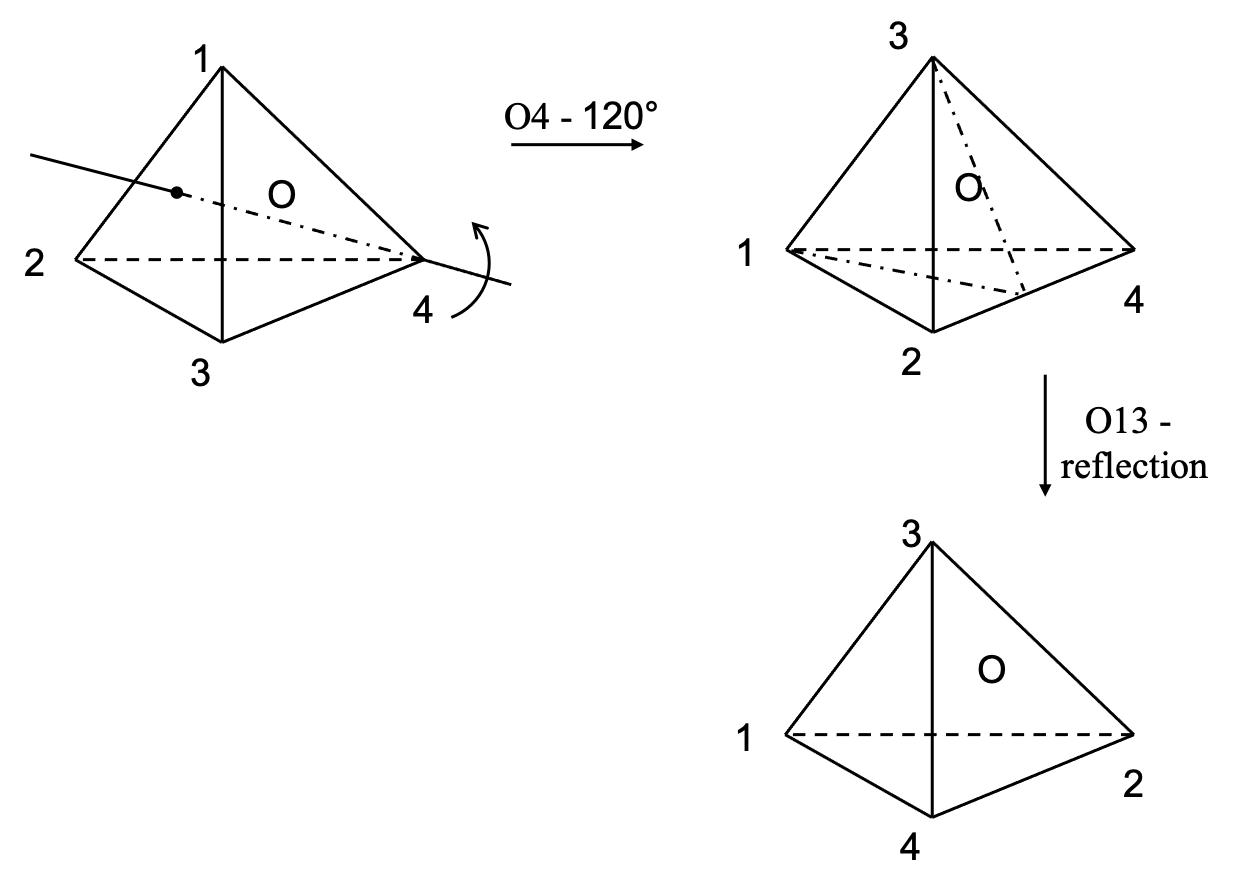
\includegraphics[scale=0.4]{img/S4.png}
 %\captionsetup{labelformat=empty}
 \caption{Improper congruence}
 \label{fig:S4}
\end{figure}

For every element in $A_4$, there is such a improper congruence by reflection. In total 12:

3142, 2341, 1432, 1324, 4231, 3214, 4123, 2413, 2134, 3421, 4312, 1243

Although there are other 2 reflection surfaces, they don't generate new transformations, as there are $4! = 24$ permutations for 4 points. All the 24 transformations of proper and improper congruences are corresponding to the elements in $S_4$.

\item {Proof that cyclic groups are abelian.}

Let the generator be $a$. For any two elements, express them as the power of $a$, i.e. $a^p, a^q$ respectively. Because:

\[
a^p a^q = a^{p + q} = a^{q + p} = a^q a^p
\]

Hence it is abelian.

\item {Proof theorem that determines if a none empty subset $H$ of group $G$ forms a subgroup, if and only if:
  \begin{enumerate}[i]
  \item For all $a, b \in H$, the product $ab \in H$;
  \item For all element $a \in H$, its reverse $a^{-1} \in H$.
  \end{enumerate}
}

First prove the sufficiency. Condition i ensures $H$ is closed on multiplication. The associativity holds for multiplication in $G$, hence also holds in $H$. Because $H$ is not empty, there exists an element $a$, based on condition ii, the corresponding $a^{-1}$ is also in $H$. And from condition i, $aa^{-1} = e \in H$ holds. Therefore $H$ is a subgroup.

Next prove the necessity. If $H$ forms a subgroup, then condition i is true obviously. For condition ii, since $H$ is a group, there exits the unit element $e'$, such that for every element $a$ in $H$, equation $e'a = a$ holds. As both $e'$ and $a$ are in $G$, we say $e'$ is a solution to equation $ya = a$ in $G$. However, there is only one solution in $G$ for this equation, which is the unit $e$ of $G$, hence $e' = e \in H$.

As $H$ is a group, equation $ya = e$ has solution $a'$ in $H$. While $a'$ is also the solution of this equation in $G$. However, the unique solution to this equation in $G$ is $a^{-1}$. Therefore, $a' = a^{-1} \in H$.

\item {List the left cosets for $H$ in below figure.}

\begin{figure*}[htbp]
\centering
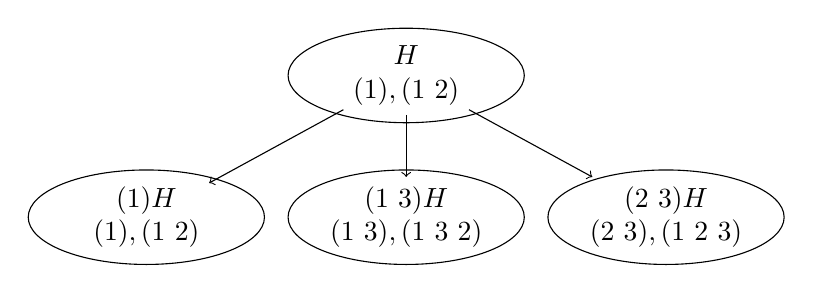
\begin{tikzpicture}[scale=0.6]
\draw (0, 3) circle[x radius=2.5cm, y radius=1cm] node[align=center] (H) {$H$ \\ $(1), (1\ 2)$}
      (-5.5, 0) circle[x radius=2.5cm, y radius=1cm] node[align=center] (H1) {$(1) H$ \\ $(1), (1\ 2)$}
      (0, 0) circle[x radius=2.5cm, y radius=1cm] node[align=center] (H13) {$(1\ 3) H$ \\ $(1\ 3), (1\ 3\ 2)$}
      (5.5, 0) circle[x radius=2.5cm, y radius=1cm] node[align=center] (H23) {$(2\ 3) H$ \\ $(2\ 3), (1\ 2\ 3)$};
\draw[->] (H) edge (H1)
          (H) edge (H13)
          (H) edge (H23);
\end{tikzpicture}
\end{figure*}

Multiply the subgroup $H = \{(1), (1\ 2)\}$ from left with (1), (1 3), and (2 3) gives:

\blre
(1) H & = & \{(1), (1\ 2)\} \\
(1\ 3) H & = & \{(1\ 3), (1\ 3\ 2)\} \\
(2\ 3) H & = & \{(2\ 3), (1\ 2\ 3)\} \\
\elre

\item {Today is Sunday, what day it will be after $2^{100}$ days?}

There are 7 days in a week. According to the Fermat's little theorem, $2^{7-1} \equiv 1 \mod 7$. We have:

\blre
2^{100} = 2^{16 \times 6 + 4} & \equiv & 1 \times 2^4 \mod 7 \\
  & \equiv & 16 \mod 7 \\
  & \equiv & 2 \mod 7 \\
\elre

Therefore, it will be Tuesday.

\item {Given two strings (character string or list), write a program to test if they form the same necklace.}

Given two strings $S_1, S_2$ with the same length, we can duplicate $S_1$ and append it after itself, then examine whether $S_2$ is the sub-string of $S_1S_1$. If yes, then they can form the same necklace.

\[
eqiv(S_1, S_2) = S_2 \subset (S_1 \doubleplus S_1)
\]

\item {Write a program to realize Eratosthenes sieve algorithm.}

For all natural numbers from 2, pick the next as a prime, then remove all its multiplicands. Then do this repeatedly. Here is an example Haskell program:

\lstset{language=Haskell, frame=single}
\begin{lstlisting}
primes = sieve [2..] where
    sieve (x:xs) = x : sieve [y | y <- xs, y `mod` x > 0]
\end{lstlisting}

The following are the example Python and Java programs.

\lstset{language=Python}
\begin{lstlisting}
def odds():
    i = 3
    while True:
        yield i
        i = i + 2

class prime_filter(object):
    def __init__(self, p):
        self.p = p
        self.curr = p

    def __call__(self, x):
        while x > self.curr:
            self.curr += self.p
        return self.curr != x

def sieve():
    yield 2
    iter = odds()
    while True:
        p = next(iter)
        yield p
        iter = filter(prime_filter(p), iter)

list(islice(sieve(), 100))
\end{lstlisting}

\lstset{language=Java}
\begin{lstlisting}
public class Prime {
    private static LongPredicate sieves = x -> true; // initialize sieve as id
    public final static long[] PRIMES = LongStream
        .iterate(2, i -> i + 1)
        .filter(i -> sieves.test(i))
        .peek(i -> sieves = sieves.and(v -> v % i != 0)) // update, chain the sieve
        .limit(100)                 // take first 100
        .toArray();
}
\end{lstlisting}

\item{Extend the idea of Eratosthenes sieve algorithm, write a program to generate Euler $\upphi$ function values for all numbers from 2 to 100.}

When generate prime numbers within $n$ with the sieve of Eratosthenes, we can update the Euler $\upphi$ function list by every prime numbers found so far. The list is initialized with all elements start from 1. For every prime number $p$, the corresponding $\upphi(p) = p(1 - \dfrac{1}{p}) = p - 1$. All the multiplicands of $p$ need multiply with this value. However, it is not enough as $\upphi(p^2) = p^2(1 - \dfrac{1}{p}) = p \upphi(p)$. Next we need multiply all the Euler function value for multiplicands of $p^2$ by $p$, and repeat for multiplicands of $p^3$ and so on until $p^m$ exceeds $n$. Below is the algorithm of this idea.

\begin{algorithmic}
\Function{Euler-Totient}{$n$}
  \State $\upphi \gets \{1, 1, ..., 1\}$ \Comment{1 to $n$}
  \State $P \gets \{2, 3, ..., n\}$ \Comment{sieve input}
  \While{$P \neq \varnothing$}
    \State $p \gets P[0]$
    \State $P \gets \{x | x \in P[1...], x \bmod p \neq 0\}$
    \State $p' \gets p$
    \Repeat
      \For{$i \gets$ from $p'$ to $n$ step $p'$}
        \If{$p' = p$}
          \State $\upphi[i] \gets \upphi[i] \times (p - 1)$
        \Else
          \State $\upphi[i] \gets \upphi[i] \times p$
        \EndIf
      \EndFor
      \State $p' \gets p' \times p$
    \Until{$p' > n$}
  \EndWhile
  \State \Return $\upphi$
\EndFunction
\end{algorithmic}

\item {Write a program to realize fast modular multiplication, and Fermat's primality test.}

Our idea is to realize the fast modular multiplication with the similar approach when calculate power.

\[
x^y =
\begin{cases}
y \text{ is even}: & x^{\lfloor y / 2 \rfloor} \\
y \text{ is odd}: & x \cdot x^{\lfloor y / 2 \rfloor} \\
\end{cases}
\]

Based on this, we can change it to modular multiplication as below:

\begin{algorithmic}
\Function{Mod-Exp}{$x, y, n$}
  \If{$y = 0$}
    \State \Return 1
  \EndIf
  \State $z \gets$ \Call{Mod-Exp}{$x, \lfloor y /2 \rfloor, n$}
  \If{$y$ is even}
    \State \Return $z^2 \bmod n$
  \Else
    \State \Return $x \cdot z^2 \bmod n$
  \EndIf
\EndFunction
\end{algorithmic}

With Fermat's little theorem, we can realize the primality test with some selected 'witnesses':

\begin{algorithmic}
\Function{primality}{$n$}
  \State random select $k$ positive numbers $a_1, a_2, ..., a_k < n$
  \If{$a_i^{n-1} \equiv 1 \mod n$, for all $i = 1, 2, ..., k$}
    \State \Return prime
  \Else
    \State \Return composite
  \EndIf
\EndFunction
\end{algorithmic}

\item {Prove the theorem that the two cancellation rules hold in a nonzero ring (ring without zero divisor).}

\begin{proof}
Suppose there is no zero divisor in $R$. Because
\[
  ab = ac \Rightarrow a(b - c) = 0
\]

as no zero divisor, hence:

\[
  a \neq 0, ab = ac \Rightarrow b - c = 0 \Rightarrow b = c
\]

Similarly,

\[
  a \neq 0, ba = ca \Rightarrow b = c
\]

Therefore, both cancellation rules hold in $R$. Reversely, suppose the first cancellation rule hold in $R$. Because:

\[
  ab = 0 \Rightarrow ab = a0
\]

Based on the assumption,

\[
  a \neq 0, ab = 0 \Rightarrow b = 0
\]

Hence $R$ does not have zero divisor. We can make the similar prove when the second cancellation rule holds.
\end{proof}

\item {Prove that, all real numbers in the form of $a + b \sqrt{2}$, where $a, b$ are integers form a integral domain under the normal addition and multiplication.}

\begin{proof}
We need verify three things:

  \begin{enumerate}[i]
  \item The commutative law for multiplication holds.
    \bre
      (a + b \sqrt{2})(c + d \sqrt{2}) & = & ac + 2bd + (ad + bc)\sqrt{2} \\
        & = & (c + d \sqrt{2})(a + b \sqrt{2})
    \ere
  \item There is unit 1 for multiplication.
    \[
      1 (a + b \sqrt{2}) = (a + b \sqrt{2}) 1 = a + b \sqrt{2}
    \]
  \item No zero divisor
    \[
    (a + b \sqrt{2})(c + d \sqrt{2}) = 0 \Rightarrow a = b = 0\ \text{or}\ c = d = 0
    \]
  \end{enumerate}
\end{proof}

\item {Prove that $Q[a, b] = Q[a][b]$, where $Q[a, b]$ contains all the expressions combined with $a$ and $b$, such as $2ab, a + a^2b$ etc.}

Let us see an example first:

\[
 Q[\sqrt{2}, \sqrt{3}] = \{a + b \sqrt{2} + c \sqrt{3} + d \sqrt{6}, \text{where } a, b, c, d \in Q\}
\]

\bre
Q[\sqrt{2}][\sqrt{3}] & = & \{a + b \sqrt{3}, \text{where } a, b \in Q[\sqrt{2}]\} \\
  & = & \{a' + b' \sqrt{2} + (c + d \sqrt{2}) \sqrt{3}, \text{where } a', b', c, d \in Q\} \\
  & = & \{a' + (b' + d) \sqrt{2} + c \sqrt{3} + d \sqrt{6}, \text{where } a', b', c, d \in Q\}
\ere

\begin{proof}
\[
Q[a][b] = \{x_0 + x_1 b + x_2 b^2 + ... + x_n b^n, \text{where } x_i \in Q[a]\}
\]
$n$ is the minimum integer that polynomial $p(b) = 0$ exists. Substitute $x_i$ with the expressions in field $Q[a]$.

\bre
Q[a][b] & = & \{ y_{0,0} + y_{0,1} a + y_{0,2} a^2 + ... + y_{0,m} a^m\ + \\
        &   &   (y_{1,0} + y_{1,1} a + y_{1,2} a^2 + ... + y_{1,m} a^m) b\ + \\
        &   &   ... \\
        &   &   + (y_{n,0} + y_{n,1} a + y_{n,2} a^2 + ... + y_{n,m} a^m) b^n \}
\ere

Where $y_{i,j} \in Q$, $m$ is the minimum integer that polynomial $p(a) = 0$ exists.

Without loss of generality, we assume $m < n$ (otherwise, we let $m' = min(m, n), n' = max(m, n)$). We can further convert it as:

\bre
Q[a][b] & = & \{ y_{0,0} + y_{0,1} a + y_{1,0} b + y_{0,2} a^2 + y_{1,1} ab + y_{2,0} b^2 + ... \\
        &   &    + y_{0,m} a^m + y_{1,m-1} a^{m-1} b + ... + y_{m, 0} b^m + \\
        &   &    y_{1,m} a^m b + y_{2, m-1} a^{m-1} b^2 + ... + y_{m, 1} b^{m+1} + ... \\
        &   &    + y_{n, m} a^m b^n \}
\ere

This field is formed with all the expressions of $a, b$.
\end{proof}

\item {Prove that, for any polynomial $p(x)$ with rational coefficients, $E/Q$ is the field extension, $f$ is the $Q$-automorphism of $E$, then equation $f(p(x)) = p(f(x))$ holds.}

\begin{proof}
Because $f$ is automorphism, we have:

\[
f(x + y) = f(x) + f(y), f(ax) = f(a) f(x), f(1/x) = 1 / f(x)
\]

Further, since $f$ is $Q$-automorphism, we have:

\[
 f(x) = x, \forall x \in Q
\]

Let $p(x) = a_0 + a_1 x + ... + a_n x^n$, where $a_i \in Q$, then:

\bre
f(p(x)) & = & f(a_0 + a_1 x + ... + a_n x^n) \\
  & = & f(a_0) + f(a_1 x) + ... + f(a_n x^n) & f(x + y) = f(x) + f(y) \\
  & = & f(a_0) + f(a_1) f(x) + f(a_2) f(x)^2 + ... + f(a_n) f(x)^n & f(ax) = f(a) f(x) \\
  & = & a_0 + a_1 f(x) + a_2 f(x)^2 + ... + a_n f(x)^n & f(x) = x, \forall x \in Q \\
  & = & p(f(x)) \\
\ere
\end{proof}

\item{Taking the complex number into account, what is the splitting field for polynomial $p(x) = x^4-1$? What are the functions in its $Q$-automorphism?}

There are four roots for polynomial $x^4 -1$. They are $\pm 1, \pm i$. We can factor the polynomial to $p(x) = (x + 1)(x - 1)(x + i)( x - i)$. Actually, the splitting field of $p(x)$ is not complex number field $C$. It is too big. The splitting field is $Q[i]$.

There are two transformations in this $Q$-automorphism. One is $f(a + bi) = a - bi$, the other is the identity transformation $g(x) = x$.

\item{What's the Galois group for quadratic equation $x^2 - bx + c = 0$?}

We know the two roots for quadratic equation are:

\[
x_1, x_2 = \dfrac{b \pm \sqrt{b^2 - 4c}}{2}
\]

There are three cases: (1) there exists a rational number, such that $b^2 - 4c = r^2$. There are two rational roots (including duplicated ones) in this case; (2) No such rational number. Equation is not solvable in rational field, but there are real roots; (3) the discriminant is negative, hence the equation is not solvable in real field. But there are complex roots. Let's see the corresponding Galois groups for these three cases:

Case 1: there are two rational roots $\dfrac{b \pm r}{2}$. There is only one element in its Galois group, which is the identity automorphism $f(x) = x$.

Case 2: there are two irrational roots $\dfrac{b \pm \sqrt{d}}{2}$. There are two elements in its Galois group. One is the automorphism $f(p + q \sqrt{d}) = p - q \sqrt{d}$, where $p, q$ are rationals; the other is the identity transformation.

Case 3: There are two complex roots $\dfrac{b \pm i \sqrt{d}}{2}$. There are two elements in its Galois group. One is the automorphism $f(p + q i) = p - q i$, where $p, q$ are real numbers; the other is the identity transformation.

Actually, in case 2 and 3, their Galois groups are isomorphic in the splitting field. Note that $f(f(x)) = x$. It is isomorphic to the group of two elements ${0, 1}$ under the addition modulo 2. It is also isomorphic to the cyclic group $C_2$ or $\pmb{Z}/2\pmb{Z}$. Where the notation $\pmb{Z}/2\pmb{Z}$ means the quotation group of integers under addition $\pmb{Z}$ and its sub-group of even numbers $2\pmb{Z}$.

\item{Prove that, if $p$ is prime number, then Galois group for equation $x^p - 1$ is the ($p-1$)-cycle cyclic group $C_{p-1}$.}

The $p$ roots of $x^p - 1$ are the points along the unit circle in complex plane, i.e. $1, \omega, \omega^2, ..., \omega^{p-1}$. They can be expressed in form of $e^{2 \pi k i / p}$. The splitting field is $Q[\omega]$.

Consider automorphism $f$ as an element in Galois group $Gal(Q[\omega]/Q)$. According to the definition of automorphism, we have:

\[
f(\omega)^k = f(\omega^k) = 1 \iff \omega^k = 1
\]

It means $f(\omega)$ is also a $p$-th root of unity (a root of equation $x^p - 1 = 0$\footnote{If $p$ is not a prime number, but an integer $n$ greater than 1, then the $k$-th power of the $m$-th root is $\zeta_m^k = e^{2 \pi m k i / n}$. There may exist some $k < n$, such that $\zeta_m^k = 1$. Actually, it holds as far as $n$ divides $mk$. However, if $n$ is a prime number $p$, then $k$ can't be less than $p$, but must be multiplicand of $p$.}). Denote:

\[
f(\omega) = h_i(\omega) = \omega^{i}
\]

If $f(\omega)$ is the $i$-th root of unity, we name it as $h_i$, where $1 \leq i \leq p-1$ (why $i$ can't be 0?). In this way, we establish a one-to-one mapping from Galois group to cyclic group $C_{p-1}$:

\[
Gal(Q[\omega]/Q) \arrowto{\sigma} C_{p-1} :  \sigma(h_i) = i
\]

Where the Galois group contains $p-1$ automorphisms $\{h_1, h_2, ..., h_{p-1}\}$, hence it has the same order as the cyclic group $C_{p-1}$.

Next we prove this is a group isomorphism.

\[
(h_i \cdot h_j)(\omega) = h_i(h_j(\omega)) = h_i(\omega^j) = \omega^{ji} = \omega^{ij}
\]

hence

\[
\sigma(h_i \cdot h_j) = ij = \sigma(h_i) \cdot \sigma(h_j)
\]

And $h_1(\omega)$ is the generator of this cyclic Galois group.

\begin{mdframed}
Here are two different groups that often cause confusion. The first one is the group of integers under addition modulo $n$. It's a cyclic group, containing the residue class modulo $n$ of \{ 0, 1, 2, ..., $n - 1$\}, total $n$ elements. This group is often denoted as $\pmb{Z}/n\pmb{Z}$. It is isomorphic to the group formed with the $n$ roots of equation $x^n - 1 = 0$. The elements are the $n$-th root of unity $\{1 = \zeta_n^0, \zeta_n^1, \zeta_n^2, ..., \zeta_n^{n-1}\}$. The binary operation is multiplication.

\vspace{5mm}

The second group is integers under multiplication modulo $n$. The group elements are not all the residues from 0 to $n-1$, but all the ones coprime to $n$. The group operation is modulo multiplication. Denoted as $(\pmb{Z}/n\pmb{Z})^{\times}$. There are total $\upphi(n)$ elements, where $\upphi$ is Euler's totient function. When $n$ is prime $p$, there are $\{1, 2, ..., p-1\}$, total $p-1$ group elements. However, the multiplicative group modulo $n$ is not necessary cyclic. Luckily it is cyclic when $n$ is prime. An interesting fact is that $(\pmb{Z}/p\pmb{Z})^{\times}$ is isomorphic to the additive group $\pmb{Z}/(p-1)\pmb{Z}$.

\vspace{5mm}

This exercise tells us: For the Galois group in rational field extension, if it is generated by $n$-th root of unity, then this group is isomorphic to the multiplicative group of integers modulo $n$, i.e. $(\pmb{Z}/n\pmb{Z})^{\times}$. For example, the cubic equation $x^3 -1 = 0$ has three roots $\{1, \dfrac{-1 \pm i \sqrt{3}}{2}\}$. Its Galois group contains two automorphisms. One is $f(x) = x$, which is corresponding to $h_1(\omega) = \omega^1$; the other is $g(a + bi) = a - bi$, which is corresponding to $h_2(\omega) = \omega^2$. The effect of $h_2$ is transform the order of the three roots from $1, 2, 3$ to $1, 3, 2$.

\[
\begin{array}{l}
1 \mapsto 1^2 = 1 \\
\omega \mapsto \omega^2 \\
\omega^2 \mapsto (\omega^2)^2 = \omega^3 \omega = \omega \\
\end{array}
\]

\end{mdframed}

\item {The 5th degree equation $x^5 - 1 = 0$ is radical solvable. What's its Galois subgroup chain?}

From previous exercise, we know the 5 roots are points along the unit circle in the complex plane: \{1, $\zeta$, $\zeta^2$, $\zeta^3$, $\zeta^4$ \}, where $\zeta = e^{2 \pi i / 5} = \dfrac{\sqrt{5} - 1 + i\sqrt{10 + 2 \sqrt{5}}}{4}$. The Galois group in rational field is a cyclic group of order 4: $G(Q[\zeta]/Q) = C_4$. It is isomorphic to the multiplicative group modulo 5: $(\pmb{Z}/5\pmb{Z})^{\times} = \{1, 2, 3, 4 \}_5$. There is no intermediate field extension. The splitting field is $Q[\zeta]$. The Galois group in splitting field is $\{1\}$.

Obviously, $\{1\}$ is the normal subgroup of $C_4$. The quotient group $C_4/\{1\}$ is cyclic too. In previous exercise, we proved that cyclic group is abelian, hence the equation is radical solvable.

\end{enumerate}

\section{categories}

\begin{enumerate}
\item {Prove that the identity arrow is unique (hint: refer to the uniqueness of identity element for groups in previous chapter).}

Suppose there exists another identity arrow $id_A'$, pointed $A$ from itself: $A \arrowto{id_A'} A$.

Consider every arrow from $A$ to $B$: $A \arrowto{f} B$, from the definition of identity arrow, $f \circ id_A = f$ holds. When replace $B$ with $A$, and replace $f$ with $id_A'$, then:

\[
id_A' \circ id_A = id_A'
\]

Similar, for every arrow from $B$ to $A$: $B \arrowto{g} A$, according to the definition of identity arrow, $id_A' \circ g = g$ holds. When replace $B$ with $A$, replace $g$ with $id_A$, then:

\[
id_A' \circ id_A = id_A
\]

Summarize these two result, we obtain $id_A = id_A'$, hence the identity arrow is unique.

\item {Verify the monoid $(S, \cup, \varnothing)$ (the elements are sets, the binary operation is set union, the identity element is empty set) and $(N, +, 0)$ (elements are natural numbers, the binary operation is add, the identity element is zero) are all categories that contain only one object.}

The key idea is that every monoid is a category contains only one object. It's a bit difficult to answer: what is the object in this category? In fact, it does not matter what this object is. The object is not necessary the monoid, or any given set. It even need not contain any elements. To avoid bother with concrete object, we give it notation $\bigstar$.

Let's first see the set monoid under union. Every set as an element in the monoid $s \in S$ can be used to define an arrow:

\[
\bigstar \arrowto{s} \bigstar
\]

Note there is no any inner structure (of the monoid) involved. The arrow composition is exactly set union.

\begin{center}
\begin{tikzpicture}
  \matrix (m) [matrix of math nodes,
               row sep=3em, column sep=4em, minimum width=2em]{
     & \bigstar & \\
     \bigstar & & \bigstar \\};
  \path[-stealth]
    (m-2-1) edge node [above] {$s_1$} (m-1-2)
    (m-1-2) edge node [above] {$s_2$} (m-2-3)
    (m-2-1) edge node [below] {$s_1 \circ s_2 = s_1 \cup s_2$} (m-2-3);
\end{tikzpicture}
\end{center}

Because set union is associative, the arrows is also associative. The empty set is the unit of this monoid, it defines the identity arrow. As the empty set unions any set equals to that set itself. It serves as the identity arrow. The set monoid under union does form a category contains only one object.

\begin{figure}[htbp]
\centering
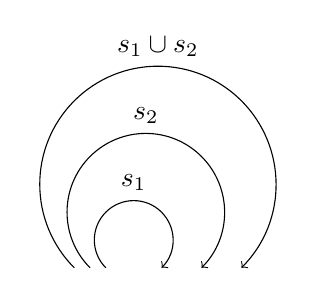
\begin{tikzpicture}
\path (0, 0) node (obj) {$\bigstar$};
\draw[->] (-0.2, 0) arc[radius=5mm, start angle=225, end angle=-45] node[pos=0.5, above]{$s_1$};
\draw[->] (-0.4, 0) arc[radius=10mm, start angle=225, end angle=-45] node[pos=0.5, above]{$s_2$};
\draw[->] (-0.6, 0) arc[radius=15mm, start angle=225, end angle=-45] node[pos=0.5, above]{$s_1 \cup s_2$};
\end{tikzpicture}
\captionsetup{labelformat=empty}
\end{figure}

Next let us see the additive monoid for natural numbers. Every number $n$ can define an arrow:

\[
\bigstar \arrowto{n} \bigstar
\]

The arrow composition is addition. Since addition is associative, hence arrow composition is also associative. Zero, 0 defines the identity arrow. This is because 0 adds to any number equals to this number itself. Therefore, the additive monoid for natural numbers does form a category.

\begin{figure}[htbp]
\centering
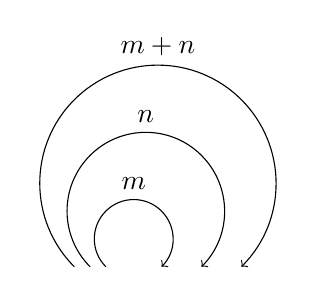
\begin{tikzpicture}
\path (0, 0) node (obj) {$\bigstar$};
\draw[->] (-0.2, 0) arc[radius=5mm, start angle=225, end angle=-45] node[pos=0.5, above]{$m$};
\draw[->] (-0.4, 0) arc[radius=10mm, start angle=225, end angle=-45] node[pos=0.5, above]{$n$};
\draw[->] (-0.6, 0) arc[radius=15mm, start angle=225, end angle=-45] node[pos=0.5, above]{$m + n$};
\end{tikzpicture}
\captionsetup{labelformat=empty}
\end{figure}


\item {In chapter 1, we introduced Peano's axioms for natural numbers and isomorphic structures to Peano arithmetic, like the linked-list etc. They can be described in categories. This was found by German mathematician Richard Dedekind although the category theory was not established by his time. We named this category as Peano category, denoted as $\pmb{Pno}$. The objects in this category is $(A, f, z)$, where $A$ is a set, for example natural numbers $N$; $f: A \to A$ is a successor function. It is $succ$ for natural numbers; $z \in A$ is the starting element, it is zero for natural numbers. Given any two Peano objects $(A, f, z)$ and $(B, g, c)$, define the morphism from $A$ to $B$ as:

\[
A \arrowto{\phi} B
\]

It satisfies:

\[
\phi \circ f = g \circ \phi \quad \text{and} \quad \phi(z) = c
\]

Verify that $\pmb{Pno}$ is a category.}

An object in Peano category is a tuple of $(A, f, z)$. An arrow is a map $\phi$ that preserve the tuple structure. Arrow composition is function composition:

\[ \begin{array}{l}
A \arrowto{\phi} B \arrowto{\psi} C \\
A \arrowto{\psi \circ \phi} C
\end{array}\]

Because function composition is associative, hence arrow composition is associative. For identity arrow:

\[
A \arrowto{id_A} A
\]

It satisfies $id_A(z) = z$, and $id_A \circ f = f \circ id_A$.

Obviously, the tuple $(\pmb{N}, succ, 0)$ is an object in Peano category. It's interesting that, for every object $(A, f, z)$ in Peano category, there is a unique arrow:

\[
(\pmb{N}, succ, 0) \arrowto{\sigma} (A, f, z)
\]

where:

\[
\sigma(n) = f^n(z)
\]

which maps any natural number $n$ to the result of applying $f$ to $z$ for $n$ times.

\item {For the list functor, define the arrow map with $foldr$.}

It's about to define list map with $foldr$ essentially:

\[
fmap\ f = foldr\ f\ Nil
\]

\item {Verify that the composition of maybe functor and list functor $\mathbf{Maybe} \circ \mathbf{List}$ and $\mathbf{List} \circ \mathbf{Maybe}$ are all functors.}

We only prove $\mathbf{Maybe} \circ \mathbf{List}$ is a functor. The other proof is similar. Any object $A$ is sent to $\mathbf{Maybe} (\mathbf{List}\ A)$. For arrows, let us first see the case of identity arrow:

\bre
(\mathbf{Maybe} \circ \mathbf{List})\ id & = & \mathbf{Maybe} (\mathbf{List}\ id) & \text{functor composition} \\
 & = & \mathbf{Maybe}\ id & \text{identity arrow for list functor} \\
 & = & id & \text{identity arrow for maybe functor} \\
\ere

Next is about arrow composition:

\bre
(\mathbf{Maybe} \circ \mathbf{List})\ (f \circ g) & = & \mathbf{Maybe} (\mathbf{List}\ (f \circ g)) & \text{functor composition} \\
 & = & \mathbf{Maybe} ((\mathbf{List}\ f) \circ (\mathbf{List}\ g)) & \text{composition for list functor} \\
 & = & (\mathbf{Maybe}\ (\mathbf{List}\ f)) \circ (\mathbf{Maybe}\ (\mathbf{List}\ g)) & \text{composition for maybe functor} \\
 & = & ((\mathbf{Maybe} \circ \mathbf{List})\ f) \circ ((\mathbf{Maybe} \circ \mathbf{List})\ g) & \text{functor composition} \\
\ere

\item {Proof that the composition for any functors $\mathbf{G} \circ \mathbf{F}$ is still a functor.}

Similar to previous exercise, we need prove functor composition satisfies identity arrow and arrow composition. First for identity arrow:

\bre
(\mathbf{G} \circ \mathbf{F})\ id & = & \mathbf{G} (\mathbf{F}\ id) & \text{functor composition} \\
 & = & \mathbf{G}\ id & \text{identity arrow for functor $\mathbf{F}$} \\
 & = & id & \text{identity arrow for functor $\mathbf{G}$} \\
\ere

Then for arrow composition:

\bre
(\mathbf{G} \circ \mathbf{F})\ (\phi \circ \psi) & = & \mathbf{G} (\mathbf{F}\ (\phi \circ \psi)) & \text{functor composition} \\
 & = & \mathbf{G} ((\mathbf{F}\ \phi) \circ (\mathbf{F}\ \psi)) & \text{arrow composition for functor $\mathbf{F}$} \\
 & = & (\mathbf{G}\ (\mathbf{F}\ \phi)) \circ (\mathbf{G}\ (\mathbf{F}\ \psi)) & \text{arrow composition for functor $\mathbf{G}$} \\
 & = & ((\mathbf{G} \circ \mathbf{F})\ \phi) \circ ((\mathbf{G} \circ \mathbf{F})\ \psi) & \text{functor composition} \\
\ere

\item {Give an example functor for preset.}

The functor for preset category is a monotone function.

\item {For the binary tree defined in chapter 2, define the functor for it.}

Consider an object $A$ in set total function category, the binary tree functor sends it to:

\lstset{language=Haskell, frame=none}
\begin{lstlisting}
data Tree A = Empty | Branch (Tree A) A (Tree A)
\end{lstlisting}

For arrow $A \arrowto{f} B$, the binary tree functor maps it to:

\bre
fmap\ f\ Empty & = & Empty \\
fmap\ f\ (Branch\ l\ x\ r) & = & Branch\ (fmap\ f\ l)\ (f\ x)\ (fmap\ f\ r) \\
\ere

Or we can use the $mapt$ defined in chapter 2:

\[
fmap = mapt
\]

\item{For any two objects in a poset, what is their product? what is their coproduct?}

In chapter 3, we mentioned any poset is a category, every element is the poset is an object, there is at most one arrow between two objects (the arrow exits if they have ordering relation). For two elements (objects) $a$ and $b$, if they have arrows both to the up and down stream, then:

\[
\text{meet}\ a \land b \quad \quad \quad \text{join}\ a \lor b
\]

is the

\[
\text{product} \quad \quad \quad \text{coproduct}
\]

for this pair of objects.

Where meet is the least upper bound (also called supremum) of the two objects, and join is the greatest lower bound (infimum) of them. In general, the join and meet of a subset of a partially ordered set need not exist, hence the product and coproduct of a poset need not exist too.

% https://en.wikipedia.org/wiki/Join_and_meet
%In mathematics, specifically order theory, the join and meet of a subset S of a partially ordered set P are respectively the supremum (least upper bound) of S, denoted ⋁S, and infimum (greatest lower bound) of S, denoted ⋀S. In general, the join and meet of a subset of a partially ordered set need not exist. Join and meet are dual to one another with respect to order inversion.

%\item {考虑集合范畴$\pmb{Set}$,积中的两个箭头$fst, snd$是右消去(epic)的么?和中的两个箭头$left, right$是左消去(monic)的么?}
\item {Prove the absorption law for coproduct, and verify the coproduct functor satisfies composition condition.}

The absorption law for coproduct states:

\[
[p, q] \circ (f + g) = [p \circ f, q \circ g]
\]

\begin{proof}
\blre
  & [p, q] \circ (f + g)  \\
= & [p, q] \circ [left \circ f, right \circ g] & \text{definition of $+$} \\
= & [[p, q] \circ (left \circ f), [p, q] \circ (right \circ g)] & \text{fusion law} \\
= & [[p, q] \circ left \circ f, [p, q] \circ right \circ g] & \text{associative} \\
= & [p \circ f, q \circ g] & \text{cancellation law} \\
\elre
\end{proof}

The composition condition for coproduct states:

\[
 (f + g) \circ (f' + g') = f \circ f' + g \circ g'
\]

\begin{proof}
Let $p = left \circ f$, and $q = right \circ g$

\blre
  & (f + g) \circ (f' + g') \\
= & [left \circ f, right \circ g] \circ (f' + g') & \text{definition of $+$} \\
= & [p, q] \circ (f' + g') & \text{substitute with $p, q$} \\
= & [p \circ f', q \circ g'] & \text{absorption law} \\
= & [left \circ f \circ f', right \circ g \circ g'] & \text{substitute $p, q$ back} \\
= & [left \circ (f \circ f'), right \circ (g \circ g')] & \text{associative law} \\
= & f \circ f' + g \circ g' & \text{reverse of $+$} \\
\elre
\end{proof}

\item{Prove that $swap$ satisfies the natural transformation condition $(g \times f) \circ swap = swap \circ (f \times g)$}

For $A \arrowto{f} C$ and $B \arrowto{g} D$, we need prove the below diagram commutes.

\begin{center}
\begin{tikzpicture}
  \matrix (m) [matrix of math nodes,
               row sep=3em, column sep=5em, minimum width=2em]{
     (A, B) & (B, A) \\
     (C, D) & (D, C) \\};
  \path[-stealth]
    (m-1-1) edge node [above] {$swap_{A, B}$} (m-1-2)
    (m-2-1) edge node [below] {$swap_{C, D}$} (m-2-2)
    (m-1-1) edge node [left] {$f \times g$} (m-2-1)
    (m-1-2) edge node [right] {$g \times f = swap\ f \times g$} (m-2-2);
\end{tikzpicture}
\end{center}

\begin{proof}
\blre
  & ((g \times f) \circ swap)\ (A, B) \\
= & (g \times f)\ (swap\ (A, B)) & \text{definition of composition} \\
= & (g \times f) \circ (B, A) & \text{definition of $swap$} \\
= & (g\ B, f\ A) & \text{product of arrows} \\
= & (D, C) & \text{definition of $g, f$} \\
= & swap\ (C, D) & \text{reverse of $swap$ definition} \\
= & swap\ (f\ A, g\ B) & \text{reverse of $f, g$ definition} \\
= & swap\ ((f \times g)\ (A, B)) & \text{product of arrow} \\
= & (swap \circ (f \times g))\ (A, B) & \text{reverse of composition} \\
\elre
\end{proof}

\item {Prove that the polymorphic function $length$ is a natural transformation. It is defined as the following:
\[
\begin{array}{l}
length : [A] \to Int \\
length\ [] = 0 \\
length\ (x:xs) = 1 + length\ xs
\end{array}
\]
}

For any object $A$, the arrow $length$ indexed by $A$ is:

\[
[A] \arrowto{length_A} \mathbf{K}_{Int}\ A
\]

where $\mathbf{K}_{Int}$ is constant functor. It sends every object to $Int$, and sends every arrow to identity arrow $id_{int}$. For arrow $A \arrowto{f} B$, we need prove below diagram commutes.

\begin{center}
\begin{tikzpicture}
  \matrix (m) [matrix of math nodes,
               row sep=3em, column sep=5em, minimum width=2em]{
     A & \lbrack A \rbrack & \mathbf{K}_{Int}\ A \\
     B & \lbrack B \rbrack & \mathbf{K}_{Int}\ B \\};
  \path[-stealth]
    (m-1-1) edge node [left] {$f$} (m-2-1)
    % square
    (m-1-2) edge node [above] {$length_A$} (m-1-3)
    (m-2-2) edge node [below] {$length_B$} (m-2-3)
    (m-1-2) edge node [left] {$\mathbf{List}(f)$} (m-2-2)
    (m-1-3) edge node [right] {$\mathbf{K}_{Int}(f)$} (m-2-3);
\end{tikzpicture}
\end{center}

From the definition of constant functor, this diagram is equivalent to:

\begin{center}
\begin{tikzpicture}
  \matrix (m) [matrix of math nodes,
               row sep=3em, column sep=5em, minimum width=2em]{
     A & \lbrack A \rbrack & Int \\
     B & \lbrack B \rbrack & Int \\};
  \path[-stealth]
    (m-1-1) edge node [left] {$f$} (m-2-1)
    % square
    (m-1-2) edge node [above] {$length_A$} (m-1-3)
    (m-2-2) edge node [below] {$length_B$} (m-2-3)
    (m-1-2) edge node [left] {$\mathbf{List}(f)$} (m-2-2)
    (m-1-3) edge node [right] {$id$} (m-2-3);
\end{tikzpicture}
\end{center}

We are about to prove:

\[
id \circ length_{A} = length_{B} \circ \mathbf{List}(f)
\]

Which means: $length_{A} = length_{B} \circ \mathbf{List}(f)$


\begin{proof}
Use mathematical induction, we first consider the empty list case:

\blre
  & length_B \circ \mathbf{List}(f) [] \\
= & length_B [] & \text{definition of list functor} \\
= & 0 & \text{definition of $length$} \\
= & length_A\ [] & \text{reverse of $length$ definition}
\elre

Next suppose $length_B \circ \mathbf{List}(f)\ as = length_A\ as$ holds, we have:

\blre
  & length_B \circ \mathbf{List}(f) (a:as) \\
= & length_B\ (f(a) : \mathbf{List}(f)\ as) & \text{definition of list functor} \\
= & 1 + length_B\ (\mathbf{List}(f)\ as) & \text{definition of $length$} \\
= & 1 + length_B\ \circ \mathbf{List}(f)\ as & \text{arrow composition} \\
= & 1 + length_A\ as & \text{induction assumption} \\
= & length_A\ (a:as) & \text{reverse of $length$ definition}
\elre
\end{proof}

\item {Natural transformation is composable. Consider two natural transformations $\mathbf{F} \arrowto{\phi} \mathbf{G}$ and $\mathbf{G} \arrowto{\psi} \mathbf{H}$. For any arrow $A \arrowto{f} B$, draw the diagram for their composition, and list the commutative condition.}

\begin{center}
\begin{tikzpicture}
  \matrix (m) [matrix of math nodes,
               row sep=3em, column sep=5em, minimum width=2em]{
     \mathbf{F}A & \mathbf{G}A & \mathbf{H}A \\
     \mathbf{F}B & \mathbf{G}B & \mathbf{H}B \\};
  \path[-stealth]
    (m-1-1) edge node [left] {$\mathbf{F}(f)$} (m-2-1)
    (m-1-1) edge node [above] {$\phi_A$} (m-1-2)
    (m-2-1) edge node [below] {$\phi_B$} (m-2-2)
    (m-1-2) edge node [above] {$\psi_A$} (m-1-3)
    (m-2-2) edge node [below] {$\psi_B$} (m-2-3)
    (m-1-2) edge node [left] {$\mathbf{G}(f)$} (m-2-2)
    (m-1-3) edge node [right] {$\mathbf{H}(f)$} (m-2-3);
\end{tikzpicture}
\end{center}

The commutative condition is:

\[
\mathbf{H}(f) \circ (\psi_A \circ \phi_A) = (\psi_B \circ \phi_B) \circ \mathbf{F} (f)
\]

\item{In the poset example, we say if there exists the minimum (or the maximum) element, then the minimum (or the maximum) is the initial object (or the final object). Consider the category of all posets $\pmb{Poset}$, if there exists the initial object, what is it? If there exists the final object, what is it?}

For the $\pmb{Poset}$ category, the objects are posets, the arrows are monotone functions. For two posets $P, Q$, arrow $P \arrowto{h} Q$ means for any two ordered elements $a \leq b$ in $P$, $h(a) \leq h(b)$ holds.

The initial object in this category is the empty poset $0 = \varnothing$. There is unique arrow from it to any poset $P$:

\[
\varnothing \longrightarrow P
\]

The final object is the singleton poset $1 = \{\bigstar\}$, the order relationship is $R = \{(\bigstar, \bigstar)\}$, i.e. $\bigstar \leq \bigstar$. From any poset $P$, there is unique arrow to 1:

\bre
P & \longrightarrow & \{\bigstar\} \\
p & \mapsto & \bigstar
\ere

\item{In the Peano category $\pmb{Pno}$ (see exercise 2 in section 1), what is the initial object in form $(A, f, z)$? What is the final object?}

The initial object is $(\pmb{N}, succ, 0)$. There is unique arrow from it to any object:

\[
(\pmb{N}, succ, 0) \arrowto{\sigma} (A, f, z): \sigma(n) = f^n(z)
\]

The final object is a singleton $1 = (\{\bigstar\}, \bigstar, id)$. There is unique arrow from any object $(A, f, z)$ to the final object:

\[
(A, f, z) \arrowto{\sigma} 1 : \sigma(a) = \bigstar
\]

\item{Verify that $\pmb{Exp}$ is a category. What is the $id$ arrow and arrow composition in it?}

Let us first verify the $id$ arrow $h \arrowto{id} h$, such that the following diagram commutes:

\begin{center}
\begin{tikzpicture}
  \matrix (m) [matrix of math nodes,
               row sep=3em, column sep=5em, minimum width=2em]{
     A & A \times B & \\
     A & A \times B & C \\};
  \path[-stealth]
    (m-1-1) edge node [left] {$id_A$} (m-2-1)
    (m-1-2) edge node [left] {$id_A \times id_B$} (m-2-2)
    (m-1-2) edge node [above] {$h$} (m-2-3)
    (m-2-2) edge node [below] {$h$} (m-2-3);
\end{tikzpicture}
\end{center}

Next is the arrow composition:

The composition of $h \arrowto{i} k$ and $k \arrowto{j} m$ is $j \circ i$ such that below diagram commutes:

\begin{center}
\begin{tikzpicture}
  \matrix (m) [matrix of math nodes,
               row sep=3em, column sep=5em, minimum width=2em]{
     A & A \times B & \\
     D & D \times B & C \\
     E & E \times B & \\};
  \path[-stealth]
    (m-1-1) edge node [left] {$f$} (m-2-1)
    (m-2-1) edge node [left] {$g$} (m-3-1)
    (m-1-2) edge node [left] {$f \times id_B$} (m-2-2)
    (m-2-2) edge node [left] {$g \times id_B$} (m-3-2)
    (m-1-2) edge node [above] {$h$} (m-2-3)
    (m-2-2) edge node [above] {$k$} (m-2-3)
    (m-3-2) edge node [below] {$m$} (m-2-3);
\end{tikzpicture}
\end{center}

For arrow $h \arrowto{j} k$, it means $id_k \circ j = j = j \circ id_h$ holds. And the associative law hold for any three arrows.

\item{In the reflection law $curry\ apply = id$, what is the subscript of the $id$ arrow? Please prove it with another method.}

The subscript of the $id$ arrow is the type of the binary arrow: $A \times B \to C$.

\begin{proof}
\blre
  & curry \circ apply\ f\ a\ b \\
= & curry\ (apply\ f)\ a\ b & \text{definition of composition} \\
= & (apply\ f)\ (a, b) & \text{definition of $curry$}\\
= & f(a, b) & \text{definition of $apply$} \\
= & id_{A \times B \to C}\ f(a, b)
\elre
\end{proof}

\item{We define the equation
\[
(curry\ f) \circ g = curry(f \circ (g \times id))
\]
as the fusion law for Currying. Draw the diagram and prove it.}

\begin{center}
\begin{tikzpicture}
  \matrix (m) [matrix of math nodes,
               row sep=3em, column sep=5em, minimum width=2em]{
     D & D \times B & \\
     A & A \times B & \\
     C^B & C^B \times B & C \\};
  \path[-stealth]
    (m-1-1) edge node [left] {$g$} (m-2-1)
    (m-2-1) edge node [left] {$curry\ f$} (m-3-1)
    (m-1-2) edge node [left] {$g \times id$} (m-2-2)
    (m-1-2) edge [bend right] node {} (m-3-2)
    (m-1-2) edge node [above] {$f \circ (g \times id)$} (m-3-3)
    (m-2-2) edge node [above] {$f$} (m-3-3)
    (m-3-2) edge node [below] {$apply$} (m-3-3);
\end{tikzpicture}
\end{center}

Observe the triangle of $D \times B$, $A \times B$, and $C$. We know the arrow of $D \times B \to C$ is $f \circ (g \times id)$.

According to the definition of exponentials and transpose arrow, we have:

\[
apply \circ (curry\ f) \circ g = f \circ (g \times id)
\]

According to the universal property of $curry$ and $apply$:

\[
(curry\ f) \circ g = curry (f \circ (g \times id))
\]

\item{Draw the diagram to illustrate the reverse element axiom for group.}

The reverse element axiom can be formalized as: $m \circ (id, i) = m \circ (i, id) = e$

\begin{center}
\begin{tikzpicture}
  \matrix (m) [matrix of math nodes,
               row sep=3em, column sep=5em, minimum width=2em]{
     G & G \times G & G \\
     1 & G & 1 \\};
  \path[-stealth]
    (m-1-1) edge node [above] {$(id, i)$} (m-1-2)
    (m-1-3) edge node [above] {$(i, id)$} (m-1-2)
    (m-1-1) edge node [left] {} (m-2-1)
    (m-1-2) edge node [left] {$m$} (m-2-2)
    (m-1-3) edge node [left] {} (m-2-3)
    (m-2-1) edge node [above] {$e$} (m-2-2)
    (m-2-3) edge node [above] {$e$} (m-2-2);
\end{tikzpicture}
\end{center}

\item{Let $p$ be a prime. Use the F-algebra to define the $\alpha$ arrow for the multiplicative group for integers modulo $p$ (refer to the previous chapter for the definition of this group).}

According to the $\alpha$ arrow defined for group:

\[
\mathbf{F} A \arrowto{\alpha = e + m +i} A
\]

The multiplicative group for integers modulo $p$ is defined as:

\bre
e\ () & = & 1 & \text{1 is the unit} \\
m(a, b) & = & ab \bmod p & \text{multiplication modulo $p$} \\
i(a) & = & a^{p-2} \bmod p & \text{Fermat's little theorem $a^{p-1} \equiv 1 \mod p$} \\
\ere

\item{Define F-algebra for ring (refer to the previous chapter for definition of ring).}

The algebraic structure of ring contains three parts:
\begin{enumerate}[i]
\item Carrier object $R$, the set that carries the algebraic structure of ring;
\item Polynomial functor $\mathbf{F}A = 1 + 1 + A \times A + A \times A + A$;
\item Arrow $\mathbf{F}A \arrowto{\alpha = z + e + p + m + n} A$, consists of the unit of addition $z$, the unit of multiplication $e$, addition $p$, multiplication $m$, and negation $n$.
\end{enumerate}

These define the $F$-algebra $(R, \alpha)$ for ring. When the carrier object is integers for example, the ring is defined as below under standard arithmetic:

\[\begin{array}{l}
z\ () = 0 \\
e\ () = 1 \\
p(a, b) = a + b \\
m(a, b) = ab \\
n(a) = -a \\
\end{array}\]

\item{What is the $id$ arrow for F-algebra category? What is the arrow composition?}

The $id$ arrow is the homomorphism from $F$-algebra $(A, \alpha)$ to itself. The arrow composition is the composition of $F$-morphisms. The arrow between carrier object $A \arrowto{f} B \arrowto{g} C$ makes the following diagram commute:

\begin{center}
\begin{tikzpicture}
  \matrix (m) [matrix of math nodes,
               row sep=3em, column sep=5em, minimum width=2em]{
     \mathbf{F} A & \mathbf{F} B & \mathbf{F} C \\
     A & B & C \\};
  \path[-stealth]
    (m-1-1) edge node [left] {$\alpha$} (m-2-1)
    (m-1-2) edge node [left] {$\beta$} (m-2-2)
    (m-1-3) edge node [left] {$\gamma$} (m-2-3)
    (m-1-1) edge node [above] {$\mathbf{F}(f)$} (m-1-2)
    (m-1-2) edge node [above] {$\mathbf{F}(g)$} (m-1-3)
    (m-2-1) edge node [below] {$f$} (m-2-2)
    (m-2-2) edge node [below] {$g$} (m-2-3);
\end{tikzpicture}
\end{center}

\[
  g \circ f \circ \alpha = \gamma \circ \mathbf{F}(g) \circ \mathbf{F}(f) = \gamma \circ \mathbf{F}(g \circ f)
\]

\item{Someone write the natural number like functor as the below recursive form. What do you think about it?
\begin{lstlisting}
data NatF A = ZeroF | SuccF (NatF A)
\end{lstlisting}
}

No, such definition does not work. Consider carrier object $A$, Functor $\mathbf{NatF}$ is recursive, it does not send $A$ to a determined object. In fact, we expect it is mapped to a object in Peano category $(A, f, z)$.

\item{We can define an $\alpha$ arrow for $\mathbf{NatF} Int \to Int$, named $eval$:
\[
\begin{array}{l}
eval : \mathbf{NatF} Int \to Int \\
eval\ ZeroF = 0 \\
eval\ (SuccF\ n) = n + 1 \\
\end{array}
\]
We can recursively substitute $A' = \mathbf{NatF} A$ to functor $\mathbf{NatF}$ by $n$ times. We denote the functor obtained as $\mathbf{NatF}^n A$. Can we define the following $\alpha$ arrow?
\[
\begin{array}{l}
eval : \mathbf{NatF}^n Int \to Int \\
\end{array}
\]
}

\bre
eval & : &\mathbf{NatF}^n Int \to Int \\
eval\ ZeroF & = & 0 & \text{$ZeroF$ is an object of $\mathbf{NatF}^n Int$}\\
eval\ (SuccF\ ZeroF) & = & 1 & \text{$ZeroF$ is an object of $\mathbf{NatF}^{n-1} Int$}\\
eval\ (SuccF\ (SuccF\ ZeroF)) & = & 2 & \text{$ZeroF$ is an object of $\mathbf{NatF}^{n-2} Int$}\\
... \\
eval\ (SuccF^{n-1}\ ZeroF) & = & n - 1 & \text{$ZeroF$ is an object of $\mathbf{NatF} Int$}\\
eval\ (SuccF^n\ m) & = & m + n \\
\ere

\item{For the binary tree functor $\mathbf{TreeF}\ A\ B$, fix $A$, use the fixed point to prove that $(\mathbf{Tree}\ A, [nil, branch])$ is the initial algebra}

Let $B' = \mathbf{TreeF}\ A\ B$. We recursively apply to itself, and call this result as $\mathbf{Fix}\ (\mathbf{TreeF}\ A)$.

\[
\resizebox{\textwidth}{!}{\ensuremath{
\begin{array}{rcll}
\mathbf{Fix}\ (\mathbf{TreeF}\ A) & = & \mathbf{TreeF}\ A\ (\mathbf{Fix}\ (\mathbf{TreeF}\ A)) & \text{definition of fixed point} \\
 & = & \mathbf{TreeF}\ A\ (\mathbf{TreeF}\ A (...)) & \text{expand} \\
 & = & NilF | BrF\ A\ (\mathbf{TreeF}\ A\ (...))\ (\mathbf{TreeF}\ A\ (...)) & \text{definition of binary tree functor} \\
 & = & NilF | BrF\ A\ (\mathbf{Fix}\ (\mathbf{TreeF}\ A))\ (\mathbf{Fix}\ (\mathbf{TreeF}\ A)) & \text{reverse of fixed point} \\
\end{array}
}}
\]

Compare with the definition of $Tree A$:

\begin{lstlisting}
data Tree A = Nil | Br A (Tree A) (Tree A)
\end{lstlisting}

Hence $\mathbf{Tree}\ A = \mathbf{Fix}\ (\mathbf{TreeF}\ A)$. The initial algebra is $(\mathbf{Tree}\ A, [nil, branch])$.

\end{enumerate}

\section{Fusion}

\begin{enumerate}
\item{Verify that folding from left can also be defined with $foldr$:
\[
foldl\ f\ z\ xs = foldr\ (b\ g\ a \mapsto g\ (f\ a\ b))\ id\ xs\ z
\]}

To make it easy, we rewrite it to:

\[\begin{array}{l}
foldl\ f\ z\ xs = foldr\ step\ id\ xs\ z \\
\text{where}: step\ x\ g\ a = g\ (f\ a\ x)
\end{array}\]

\blre
  & foldl\ f\ z\ [x_1, x_2, ..., x_n] \\
= & (foldr\ step\ id\ [x_1, x_2, ..., x_n])\ z \\
= & (step\ x_1 (step\ x_2 ( ... (step\ x_n\ id))) ...)\ z \\
= & (step\ x_1 (step\ x_2 ( ... (a_n \mapsto id\ (f\ a_n\ x_n)))) ...)\ z \\
= & (step\ x_1 (step\ x_2 ( ...(a_{n-1} \mapsto (a_n \mapsto id\ (f\ a_n\ x_n))\ (f\ a_{n-1}\ x_{n-1}))))...)\ z \\
= & (a_1 \mapsto (a_2 \mapsto ( ... (a_n \mapsto id\ (f\ a_n\ x_n))\ (f\ a_{n-1}\ x_{n-1})) ... (f\ a_2\ x_2)) (f\ a_1\ x_1))\ z \\
= & (a_1 \mapsto (a_2 \mapsto ( ... (a_n \mapsto f\ a_n\ x_n)\ (f\ a_{n-1}\ x_{n-1})) ... )\ (f\ a_1\ x_1))\ z \\
= & (a_1 \mapsto (a_2 \mapsto (... (a_{n-1} \mapsto f\ (f\ a_{n-1}\ x_{n-1})\ x_n)\ ...))\ (f\ a_1\ x_1))\ z \\
= & (a_1 \mapsto f\ (f\ (...(f\ a_1\ x_1)\ x_2)\ ...)\ x_n)\ z \\
= & f\ (f\ (...(f\ z\ x_1)\ x_2)\ ...)\ x_n
\elre

We can further write $f$ as an infix of $\oplus$ to highlight the difference between $foldl$ and $foldr$:

\[
foldl\ \oplus\ f\ z = ((...(z \oplus x_1)\ \oplus x_2)...)\ \oplus x_n
\]

\item{Prove the below build...foldr forms hold:
\[
\begin{array}{l}
concat\ xss = build\ (f\ z \mapsto foldr\ (xs\ x \mapsto foldr\ f\ x\ xs)\ z\ xss) \\
map\ f\ xs = build\ (\oplus\ z \mapsto foldr\ (y\ ys \mapsto (f\ y) \oplus ys)\ z\ xs) \\
filter\ f\ xs = build\ (\oplus\ z \mapsto foldr\ (x\ xs' \mapsto
  \begin{cases}
     f(x): & x \oplus xs' \\
    \text{otherwise}: & xs' \\
  \end{cases})\ z\ xs) \\
repeat\ x = build\ (\oplus\ z \mapsto let\ r = x \oplus r\ in\ r) \\
\end{array}
\]
}

First for the list $concat$:

\begin{proof}
\blre
  & build\ (f\ z \mapsto foldr\ (xs\ x \mapsto foldr\ f\ x\ xs)\ z\ xss) \\
= & (f\ z \mapsto foldr\ (xs\ x \mapsto foldr\ f\ x\ xs)\ z\ xss)\ (:)\ [] & \text{definition of $build$} \\
= & foldr\ (xs\ x \mapsto foldr\ (:)\ x\ xs)\ []\ xss & \text{$\beta$-reduction} \\
= & foldr\ \doubleplus []\ xss & \text{concatenate two lists} \\
= & concat\ xss & \text{concatenate multiple lists} \\
\elre
\end{proof}

Next for list $map$

\begin{proof}
\blre
  & build\ (\oplus\ z \mapsto foldr\ (y\ ys \mapsto (f\ y) \oplus ys)\ z\ xs) \\
= & (\oplus\ z \mapsto foldr\ (y\ ys \mapsto (f\ y) \oplus ys)\ z\ xs)\ (:)\ [] & \text{definition of $build$} \\
= & foldr\ (y\ ys \mapsto f(y) : ys)\ []\ xs & \text{$\beta$-reduction} \\
= & foldr\ (x\ ys \mapsto f(x) : ys)\ []\ xs & \text{$\alpha$ transformation, change name} \\
= & map\ f\ xs & \text{definition of list map} \\
\elre
\end{proof}

Next for $filter$

\begin{proof}
\blre
  & build\ (\oplus\ z \mapsto foldr\ (x\ xs' \mapsto
  \begin{cases}
     f(x): & x \oplus xs' \\
    \text{otherwise}: & xs' \\
  \end{cases})\ z\ xs) \\
= & (\oplus\ z \mapsto foldr\ (x\ xs' \mapsto
  \begin{cases}
     f(x): & x \oplus xs' \\
    \text{otherwise}: & xs' \\
  \end{cases})\ z\ xs)\ (:)\ [] & \text{definition of $build$} \\
= & foldr\ (x\ xs' \mapsto
  \begin{cases}
     f(x): & x : xs' \\
    \text{otherwise}: & xs' \\
  \end{cases})\ []\ xs & \text{$\beta$-reduction} \\
= & filter\ f\ xs & \text{definition of filter} \\
\elre
\end{proof}

Last for $repeat$

\begin{proof}
\blre
  & build\ (\oplus\ z \mapsto let\ r = x \oplus r\ in\ r) \\
= & (\oplus\ z \mapsto let\ r = x \oplus r\ in\ r)\ (:)\ [] & \text{definition of $build$} \\
= & (let\ r = x : r\ in\ r) & \text{$\beta$-reduction} \\
= & repeat\ x & \text{definition of repeat} \\
\elre
\end{proof}

\item{Simplify the quick sort algorithm.
\[
\begin{cases}
qsort\ [] = [] \\
qsort\ (x:xs) = qsort\ [a | a \in xs, a \leq x] \doubleplus [x] \doubleplus qsort\ [a | a \in xs, x < a] \\
\end{cases}\]
}

First, we can transform the ZF-expression to $filter$, and combine the two rounds of list filtering to one pass:

\[
\begin{cases}
qsort\ [] & = [] \\
qsort\ (x:xs) & = qsort\ as \doubleplus [x] \doubleplus qsort\ bs \\
\end{cases}
\]

where:
\[\begin{array}{l}
(as, bs) = foldr\ h\ ([], [])\ xs \\
h\ y\ (as', bs') = \begin{cases}
               y \leq x : & (y:as', bs') \\
               \text{otherwise}: & (as', y:bs') \\
\end{cases} \\
\end{array}\]

Next we further simplify the list concatenation:

\blre
  & qsort\ as \doubleplus [x] \doubleplus qsort\ bs \\
= & qsort\ as \doubleplus (x : qsort\ bs) \\
= & foldr (:)\ (x : qsort\ bs) (qsort\ as)
\elre

\item{Verify the type constraint of fusion law with category theory. Hint: consider the type of the catamorphism.}

As shown in below diagram:

\begin{center}
\begin{tikzpicture}
  \matrix (m) [matrix of math nodes,
               row sep=3em, column sep=5em, minimum width=2em]{
     \mathbf{ListF} A\ \lbrack A \rbrack & \lbrack A \rbrack \\
     \mathbf{ListF} A\ B\ & B \\};
  \path[-stealth]
    (m-1-1) edge node [left] {$\mathbf{ListF} A(h)$} (m-2-1)
    (m-1-2) edge node [right] {$h = \lbb \alpha \rbb$} (m-2-2)
    (m-1-1) edge node [above] {$(:) + []$} (m-1-2)
    (m-2-1) edge node [below] {$\alpha = f + z$} (m-2-2);
\end{tikzpicture}
\end{center}

The catamorphism $\lbb \alpha \rbb$ is abstracted to build some algebraic structure from $\alpha$, i.e. $g\ \alpha$. Where $g$ accepts the $\alpha$ arrow of an $F$-algebra, generates result of $B$. The $\alpha$ arrow is the coproduct of $f : A \to B \to B$ and $z : 1 \to B$, that the type is:

\[
g : \forall A. (\forall B. (A \to B \to B) \to B \to B)
\]

The definition of build is $build(g) = g\ (:)\ []$. It applies $g$ to the $\alpha$ arrow of the initial algebra, and builds the object of the initial algebra, which is a list of $[A]$.

\[
build : \forall A. (\forall B. (A \to B \to B) \to B \to B) \to \mathbf{List}\ A
\]

\item{Use the fusion law to optimize the expression evaluation function:
\[
eval = sum \circ map\ (product \circ (map\ dec))
\]}

\[
\resizebox{\textwidth}{!}{\ensuremath{
\begin{array}{cll}
  & eval\ es \\
= & sum (map\ (product \circ (map\ dec))\ es) & \text{function composition} \\
  & \{ \text{$sum$ in fold, $map$ in build} \} \\
= & \pmb{foldr}\ (+)\ 0\ (\pmb{build}\ (\oplus\ z\ \mapsto foldr\ (t\ ts \mapsto (f\ t) \oplus ts)\ z\ es)) & \text{let $f = product \circ (map\ dec)$} \\
= & (\oplus\ z \mapsto foldr\ (t\ ts \mapsto (f\ t) \oplus ts)\ z\ es)\ (+)\ 0 & \text{fusion law} \\
= & foldr\ (t\ ts \mapsto (f\ t) + ts)\ 0\ es & \text{$\beta$-reduction} \\
\end{array}
}}
\]

Written in point-free form as:

\[
eval = foldr\ (t\ ts \mapsto (f\ t) + ts)\ 0
\]

Next we simplify the $product \circ (map\ dec)$ part

\[
\resizebox{\textwidth}{!}{\ensuremath{
\begin{array}{cll}
  & (product \circ (map\ dec))\ t \\
= & product\ (map\ dec\ t) & \text{function composition} \\
  & \{ \text{$product$ in fold, $map$ in build} \} \\
= & \pmb{foldr}\ (\times)\ 1\ (\pmb{build}\ (\oplus\ z \mapsto foldr\ (d\ ds \mapsto (dec\ d) \oplus ds)\ z\ t)) \\
= & (\oplus\ z \mapsto foldr (d\ ds \mapsto (dec\ d) \oplus ds)\ z\ t)\ (\times)\ 1 & \text{fusion law} \\
= & foldr\ (d\ ds \mapsto (dec\ d) \times ds)\ 1\ t & \text{$\beta$-reduction} \\
= & foldr\ ((\times) \circ fork\ (dec, id))\ 1\ t & \text{let $fork(f, g)\ x = (f\ x, g\ x)$} \\
\end{array}
}}
\]

Substitute this to $f$, we obtain the final simplified result:

\[
eval = foldr\ (t\ ts \mapsto (foldr\ ((\times) \circ fork\ (dec, id))\ 1\ t) + ts)\ 0
\]

\item{How to expand all expressions from left?}

When expand from left to right, there are three options for every digit $d$:

\begin{enumerate}
\item Insert nothing. It means append $d$ to the last factor of the last sub-expression of $e_i$. Combine $f_n \doubleplus [d]$ as a new factor. For example when $e_i$ is $1 + 2$, $d$ is 3, write 3 after $1 + 2$ without inserting any symbols, we obtain a new expression $1 + 23$;

\item Insert $\times$. It means we create a new factor $[d]$, then append it to the last sub-expression of $e_i$. Combine $t_m \doubleplus [[d]]$ as a new sub-expression. For the same $1 + 2$ example, we write 3 after it, put a $\times$ between 2 and 3, hence obtain a new sub-expression $1 + 2 \times 3$;

\item Insert +. It means we create a new sub-expression $[[d]]$, then append it to $e_i$ to obtain a new expression $e_i \doubleplus [[[d]]]$. For the same $1 + 2$ example, we write 3 after it, put a + between 2 and 3, hence obtain a new expression $1 + 2 + 3$.
\end{enumerate}

We need define the append function to add an element after a list:

\[
append\ x = foldr\ (:)\ [x]
\]

Then we define a function $onLast(f)$, which applies $f$ to the last element of a list:

\[\begin{array}{l}
onLast\ f = foldr\ h\ [] \\
\text{where}: \begin{cases}
  h\ x\ [] & = [(f\ x)] \\
  h\ x\ xs & = x : xs \\
\end{cases} \\
\end{array}\]

Then we implement the above three expansion options:

\lstset{frame = none}
\begin{lstlisting}
add d exp = [((append d) `onLast`) `onLast` exp,
             (append [d]) `onLast` exp,
             (append [[d]]) exp]
\end{lstlisting}

\item{The following definition converts expression to string:
\[
str = (join\ \text{``+''}) \circ (map\ ((join\ \text{``} \times \text{''}) \circ (map\ (show \circ dec))))
\]
Where $show$ converts number to string. Function $join(c, s)$ concatenates multiple strings $s$ with delimiter $c$. For example: $join($``\#''$, [$``abc'', ``def''$]) = $``abc\#def''. Use the fusion law to optimize $str$.
}

We defined $join(ws)$ in chapter 5. It insert space between every two strings. We can extract the space as a parameter to define $join(c, s)$:

\[
join\ c = foldr\ (w\ b \mapsto foldr\ (:)\ (c:b)\ w)\ []
\]

Observe the definition of $str$. It contains embedded $(join\ c) \circ (map\ f)$ as:

\[\begin{array}{l}
str = (join\ c) \circ (map\ f) \\
\text{where}: f = (join\ d) \circ (map\ g) \\
\end{array}\]

where $c =$ `+', $d =$ `$\times$', and $g = show \circ dec$. What we need is to simplify $(join\ c) \circ (map\ f)$.

\blre
  & (join\ c) \circ (map\ f)\ es \\
  & \{ \text{$join$ in fold, $map$ in build} \} \\
= & \pmb{foldr}\ (w\ b \mapsto foldr\ (:) (c:b)\ w)\ []\ (\pmb{build}\ (\oplus\ z \mapsto foldr\ (y\ ys \mapsto (f\ y) \oplus ys)\ z\ es)) \\
  & \{ \text{fusion law} \} \\
= & (\oplus\ z \mapsto foldr\ (y\ ys \mapsto (f\ y) \oplus ys)\ z\ es))\ (w\ b \mapsto foldr\ (:)\ (c:b)\ w)\ [] \\
  & \{ \text{$\beta$-reduction} \} \\
= & foldr\ (y\ ys \mapsto foldr\ (:)\ (c:ys)\ (f\ y))\ []\ es \\
\elre

Substitute the +, $\times$, and $show \circ dec$ in, we obtain the final result:

\blre
str & = & foldr\ (x\ xs \mapsto foldr\ (:)\ (`+':xs) ( \\
    &   & \quad foldr (y\ ys \mapsto foldr\ (:)\ (`\times':ys)\ (show \circ dec\ y))\ [])\ [] \\
\elre

\end{enumerate}

\section{Infinity}

\begin{enumerate}

\item{In chapter 1, we realized Fibonacci numbers by folding. How to define Fibonacci numbers as potential infinity with $iterate$?}

\[
F = (fst \circ unzip)\ (iterate\ ((m, n) \mapsto (n, m + n))\ (1, 1))
\]

For example $take\ 100\ F$ gives the first 100 Fibonacci numbers

\item{Define $iterate$ by folding.}

Consider the infinite stream $iterate\ f\ x$. After applying $f$ to each element, and prepend $x$ as the first one, we obtain this infinite stream again. Based on this fact, we can define it as:

\[
iterate\ f\ x = x : foldr (y\ ys \mapsto (f\ y):ys)\ []\ (iterate\ f\ x)
\]

For example:

\begin{lstlisting}
take 10 $ iter (+1) 0
[0,1,2,3,4,5,6,7,8,9]
\end{lstlisting} %$

\item{Use the definition of the fixed point in chapter 4, prove $Stream$ is the fixed point of $StreamF$.}

Let $A' = \mathbf{StreamF}\ E\ A$, then apply it to itself repeatedly. We call this result $\mathbf{Fix}\ (\mathbf{StreamF}\ E)$

\bre
\mathbf{Fix}\ (\mathbf{StreamF}\ E) & = &
    \mathbf{StreamF}\ E\ (\mathbf{Fix}\ (\mathbf{StreamF}\ E)) & \text{definition of fixed point} \\
 & = & \mathbf{StreamF}\ E\ (\mathbf{StreamF}\ E\ (...)) & \text{expand recursively} \\
 & = & \mathbf{Stream}\ E\ (\mathbf{Stream}\ E\ (...)) & \text{change name} \\
 & = & \mathbf{Stream}\ E & \text{reverse of $Stream$} \\
\ere

Therefore, $Stream$ is the fixed point of $StreamF$.

\item{Define $unfold$.}

We often use $Maybe$ to define the terminate condition:

\begin{lstlisting}
unfold :: (b -> Maybe (a, b)) -> (b -> [a])
unfold f b = case f b of
                Just (a, b') -> a : unfold f b'
                Nothing -> []
\end{lstlisting}

\item{The fundamental theorem of arithmetic states that, any integer greater than 1 can be unique represented as the product of prime numbers. Given a text $T$, and a string $W$, does any permutation of $W$ exist in $T$? Solve this programming puzzle with the fundamental theorem and the stream of prime numbers.}

Our idea is to map every unique character to a prime number, for example, a $\to$ 2, b $\to$ 3, c $\to$ 5, ... Given any string $W$, no matter it contains repeated characters or not, we can convert it to a product of prime numbers:

\[
F = \prod p_c , c \in W
\]

We call it the number theory finger print $F$ of string $W$. When $W$ is empty, we define its finger print as 1. Because multiplication of integers is commutative, the finger print is same for all permutations of $W$, and according to the fundamental theorem of arithmetic, the finger print is unique. We can develop an elegant solution based on this: First, we calculate $F$ of string $W$, then slide a window of length $|W|$ along $T$ from left to right. When start, we also need to compute the finger print within this window of $T$, and compare it with $F$. If they are equal, it means $T$ contains some permutation of $W$. Otherwise, we slide the window to the right by a character. We can easily compute the updated finger print value for this new window position: divide the product by the prime number of the character slides out, and multiply the prime number of the character slides in. Whenever the finger print equals to $F$, we find a permutation. In order to map different characters to prime numbers, we can use sieve of Eratosthenes to generate a series of prime numbers. Below is the example algorithm accordingly.

\begin{algorithmic}
\Function{contains?}{$W, T$}
  \State $P \gets ana \ era \ [2, 3, ...]$ \Comment{prime numbers}
  \If{$W = \phi$}
    \State \Return True
  \EndIf
  \If{$|T| < |W|$}
    \State \Return False
  \EndIf
  \State $\displaystyle m \gets \prod P_c, c \in W$
  \State $\displaystyle m' \gets \prod P_c, c \in T[1...|W|]$
  \For{$i \gets |W| + 1$ to $|T|$}
    \If{$m = m'$}
      \State \Return True
    \EndIf
    \State $m' \gets m' \times P_{T_i} / P_{T_{i - |W|}} $
  \EndFor
  \State \Return $m = m'$
\EndFunction
\end{algorithmic}

\item{We establish the 1-to-1 correspondence between the rooms and guests. For guest $i$ in group $j$, which room number should be assigned? Which guest in which group will live in room $k$?}

Use the convention to count from zero, and use pair $(i, j)$ to denote the $j$-th guest in the $i$-th group. Let us list the first several guests and their rooms:

\begin{adjustbox}{max width=\textwidth}
\btab{c|c|c|c|c|c|c|c|c|c|c|c}
$(i, j)$ & (0, 0) & (0, 1) & (1, 0) & (2, 0) & (1, 1) & (0, 2) & (0, 3) & (1, 2) & (2, 1) & (3, 0) & ... \\
\hline
$k$ & 0 & 1 & 2 & 3 & 4 & 5 & 6 & 7 & 8 & 9 & ... \\
\hline
$i + j$ & 0 & 1 & 1 & 2 & 2 & 2 & 3 & 3 & 3 & 3 & ... \\
\etab
\end{adjustbox}

Writing down the values $i+j$, we can find the pattern. There are 1 instance of number 0, 2 instances of number 1, 3 instances of number 2, 4 instances of number 3, ... They are exactly the triangle numbers found by Pythagoreans. Let $m = i + j$, there are total $\dfrac{m(m + 1)}{2}$ grid points along the diagonals on the left-bottom side of a given grid.

For the diagonal where this point belongs to, if $m$ is odd, then the room number increases along the left up direction,  $i$ increases, and $j$ decreases; if $m$ is even, then the direction is right-bottom. Summarize the two cases gives the following result:

\[
k = \dfrac{m(m + 1)}{2} + \begin{cases} m - j: \text{$m$ is odd} \\
j: \text{$m$ is even} \\
\end{cases}
\]

Further, we can use $(-1)^m$ to simplify the conditions:

\[
k = \dfrac{m(m + 2) + (-1)^m (2j - m)}{2}
\]

\item{For Hilbert's Grand hotel, there are multiple solutions for the problem on the third day. Can you give a different numbering scheme based on the cover page of the book {\em Proof without word}?}

\begin{figure}[htbp]
\centering
\begin{tikzpicture}
  \draw[step=1, very thin, gray] (0, 0) grid (5, 5);
  \draw[->] (-0.25, 0) -- (6, 0) coordinate (x axis);
  \draw[->] (0, -0.25) -- (0, 6) coordinate (y axis);
  \foreach \x in {0, 1, 2, 3, 4, 5}
    \path (\x, -0.25) node[left] {\x};
  \foreach \y in {1, 2, 3, 4, 5}
    \path (-0.25, \y) node[below] {\y};
  \foreach \i / \x / \y in {0/0/0, 1/1/0, 2/1/1, 3/0/1, 4/0/2, 5/1/2, 6/2/2, 7/2/1, 8/2/0, 9/3/0, 10/3/1}{
    \path (\x, \y) coordinate (N\i);
    \fill (N\i) circle (1pt) node[above right=3pt of N\i] {\i};
  }
  \foreach \i in {0,...,9} {
    \pgfmathsetmacro{\j}{\i+1}
    \draw[-latex, thick] (N\i) to (N\j);
  }
\end{tikzpicture}
\caption{Another numbering scheme for infinity of infinity}
\label{fig:NNtoN2}
\end{figure}

As shown in figure \ref{fig:NNtoN2}, we count along the gnomon shaped path. There are odd number of grid points along every gnomon.

\item{Let $x = 0.9999....$, then $10x = 9.9999...$, subtract them gives $10x - x = 9$. Solving this equation gives $x = 1$. Hence $1 = 0.9999...$. Is this proof correct?}

Yes, it's correct.

\item{Light a candle between two opposite mirrors, what image can you see? Is it potential or actual infinity?}

The candle image reflects between the two mirrors endlessly, generates infinite many images. If we consider the speed of light is limited, then it is potential infinity from physics viewpoint.

\end{enumerate}

\section{Paradox}

\begin{enumerate}
\item{We can define numbers in natural language. For example ``the maximum of two digits number'' defines 99. Define a set containing all numbers that cannot be described within 20 words. Consider such an element: ``The minimum number that cannot be described within 20 words''. Is it a member of this set?}

This is an instance of Russell's paradox. Whether it is a member, all lead to contradiction.

\item{``The only constant is change'' said by Heraclitus. Is this Russell's paradox?}

Yes, this is an instance of Russell's paradox.

\item{Is the quote saying by Socrates (the beginning of chapter 7) Russell's paradox?}

Yes, it is an instance of Russell's paradox.

\item{Translate Fermat's last theorem into a TNT string.}

We need define power operation first.

\[\begin{cases}
\forall a: e(a, 0) = S0 & \text{0-th power is 1} \\
\forall a: \forall b: e(a, Sb) = a \cdot e(a, b) & \text{recursion} \\
\end{cases}\]

We can then define Fermat's last theorem atop it.

\[
\forall d: \lnot \exists a: \exists b: \exists c: \lnot (d = 0 \lor d = S0 \lor d = SS0) \to e(a, d) + e(b, d) = e(c, d)
\]

\item{Prove the associative law of addition with TNT reasoning rules.}

Surprisingly, we can prove every theorem below:

\bre
a + b + 0 & = & a + (b + 0) \\
a + b + S0 & = & a + (b + S0) \\
a + b + SS0 & = & a + (b + SS0) \\
... \\
\ere

For example:

\bre
a + b + 0 = a + b = a + (b + 0)
\ere

And:

\bre
a + b + SS0 & = & SS(a + b + 0) \\
 & = & SS(a + b) \\
 & = & a + SSb \\
 & = & a + (b + SS0) \\
\ere

However, we cannot prove: $\forall c: a + b + c = a + (b + c)$.

To do that, we has to introduce mathematical induction.

\item{Prove that $\forall a: (0 + a) = a$ with the newly added rule of induction.}

First for the case of 0:

\[
0 + 0 = 0
\]

Next suppose $(0 + a) = a$ holds, we have:

\bre
(0 + Sa) & = & S(0 + a) & \text{axiom 3} \\
  & = & Sa & \text{induction hypothesis} \\
\ere

From the rule of induction, we obtain: $\forall a: (0 + a) = a$

\end{enumerate}

\ifx\wholebook\relax \else
\begin{thebibliography}{99}

\bibitem{Lockhart2012}
Paul Lockhart. ``Measurement''. Belknap Press: An Imprint of Harvard University Press; Reprint edition 2014, ISBN: 978-0674284388

\end{thebibliography}

\expandafter\enddocument
%\end{document}

\fi
